\chapter{Manovellismi}

\section{Introduzione}

\noindent I meccanismi che si identificano col nome di 
manovellismi non sono altro, da un punto di vista cinematico, che
casi particolari di quadrilateri articolati. Essi sarebbero potuti entrare
a pieno titolo nel capitolo precedente, visto che le tecniche per
il loro studio, siano queste grafiche, analitiche o numeriche, non
differiscono da quelle che si  impiegano nell'analisi dei loro
progenitori. Il presente capitolo, dedicato esclusivamente allo studio dei
manovellismi, si giustifica valutando l'importanza industriale che 
tali meccanismi hanno
avuto e quindi anche la profondit\`a e la mole di studi che
li riguarda.
Affermiamo, senza timore di esagerare, che il
{\em manovellismo ordinario}\index{manovellismo!ordinario} o
{\em di spinta}\index{manovellismo!di spinta} \`e stato il cuore della
Rivoluzione Industriale, essendo un componente essenziale del motore a vapore.
Anche ai giorni nostri,  nel settore del trasporto su strada,
tale meccanismo entra, con numero
variabile di esemplari, praticamente in tutti i motori endotermici, tralasciando
pochissime eccezioni.

\noindent Richiamiamo la nomenclatura delle quattro cerniere
di un quadrilatero ricordando la figura \ref{fig:f_quad_schema} ovvero
prendendo visione della figura \ref{fig:quad_D_infinito}.
Ciascuna delle quattro cerniere $A$, $B$, $C$, e $D$ pu\`o essere mandata all'infinito
seguendo una precisa direzione e divenendo una di quelle
entit\`a che la geometria
definisce come {\em punti impropri} del piano.
\`E scontato che, affinch\'e una (alla volta, per il momento)
delle cerniere si trovi
infinitamente distante dalle altre tre, \`e necessario che le due aste
che vi concorrono siano a loro volta di lunghezza infinita.
\noindent Data la ovvia equivalenza cinematica dei punti $A$ e $D$ e dei punti
$B$ e $C$ si pu\`o intuire che pensare situato all'infinito l'uno o l'altro dei punti di
tali coppie produca, a livello cinematico, lo stesso effetto,
e cos\`i \`e.

\noindent Affermiamo che allo spostarsi all'infinito delle cerniere
$A$ oppure $D$ il quadrilatero d\`a origine ai {\em manovellismi ordinari}\index{manovellismo!ordinario}, naturalmente dopo avere mutato la cerniera 
``fuori uso'' con un altro tipo di vincolo, in generale costituito da un 
{\em cursore}\index{cursore} che scorre in un {\em glifo}\index{glifo}.

\noindent Nel secondo caso, quando ad andare all'infinito \`e una delle
cerniere $B$ oppure $C$, avremo i {\em manovellismi
non ordinari}.\index{manovellismo!non ordinario}
\noindent Andiamo con ordine.


\section{Il Manovellismo Ordinario}

\begin{figure}[hbt]
\centering
\begin{minipage}[b]{0.48\textwidth}
\centering
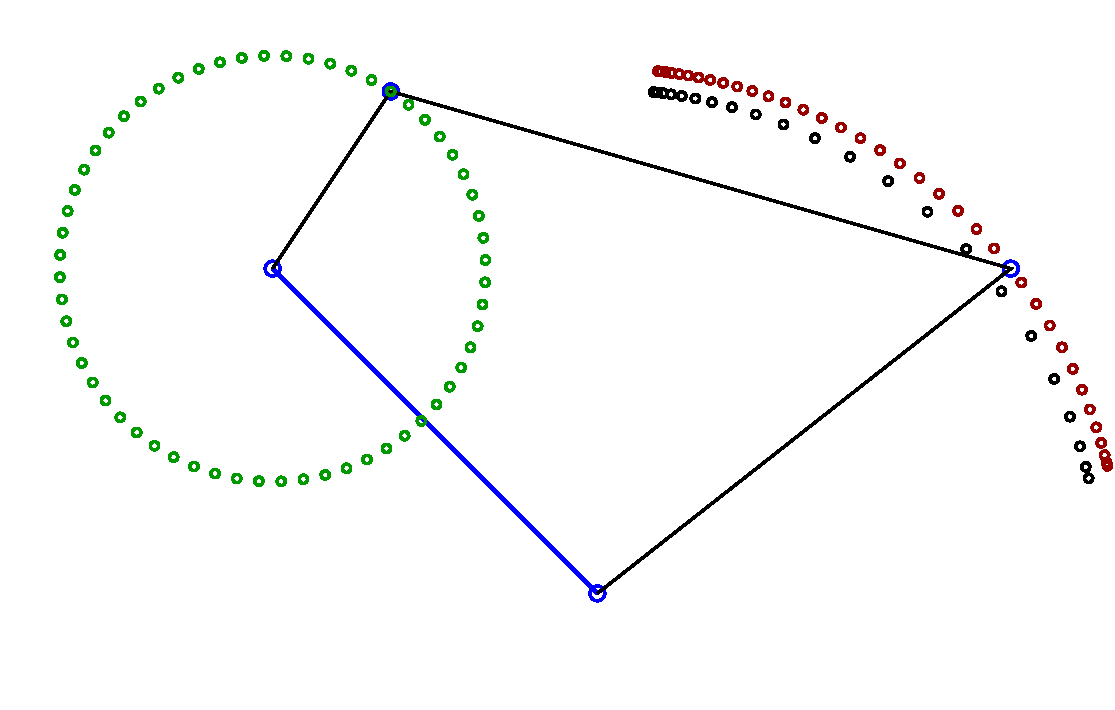
\includegraphics[width=0.95\textwidth]{part2/manovellismi/FIG/manovellismi/quad_D_infinito.pdf}
\begin{picture}(0,0)(155,-12)
\scriptsize{
\put(17,53){$A$}
\put(44,85){$B$}
\put(140,56){$C$}
\put(73,-3){$D$}
}
\end{picture}
\vskip .2mm
      \caption{\em Generico quadrilatero manovella-bilanciere.}
 \label{fig:quad_D_infinito}
\end{minipage}\hfill
\begin{minipage}[b]{0.48\textwidth}
\centering
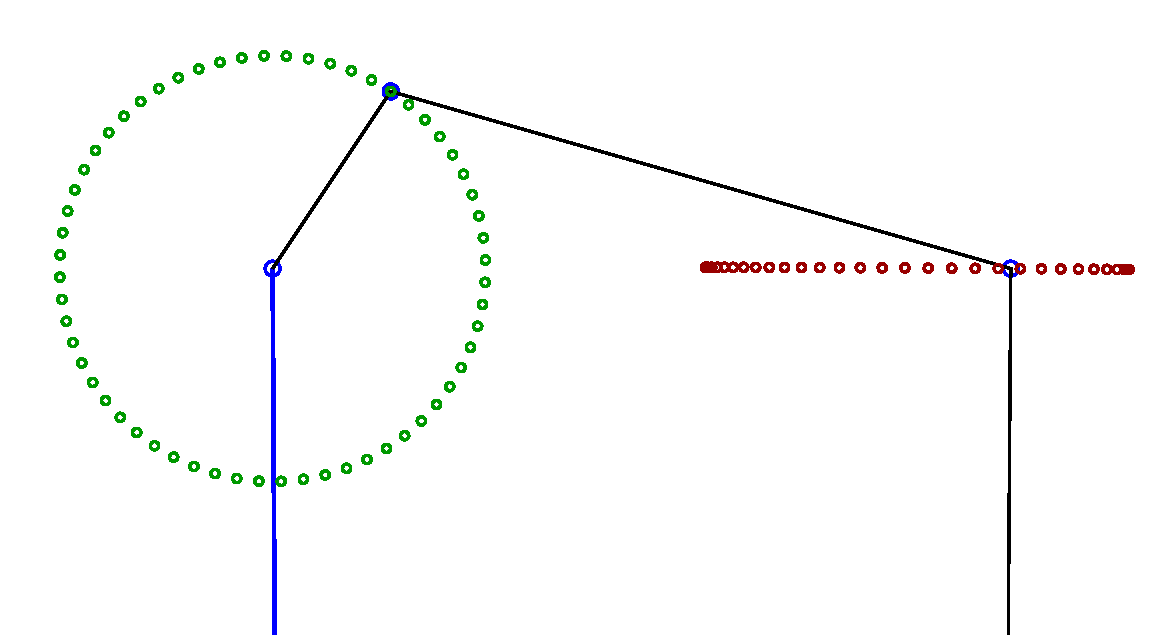
\includegraphics[width=0.95\textwidth]{part2/manovellismi/FIG/manovellismi/quad_D_infinito_man.pdf}
\begin{picture}(0,0)(155,3)
	\scriptsize{
\put(16,53){$A$}
\put(42,85){$B$}
\put(132,60){$C$}
\put(87,58){$\sigma$}
\put(93,3){$D$}
\put(100,10){\rotatebox{-90}{$\longrightarrow$}}
\put(104,3){$\infty$}
}
\end{picture}
	\caption{\em Manovellismo ordinario centrato ottenuto spostando la cerniera $D$ a distanza ``infinita''.}
     \label{fig:quad_D_infinito_man}
\end{minipage}
\end{figure}

\noindent In figura \ref{fig:quad_D_infinito_man} \`e
riportato il quadrilatero degenere che si ottiene mandando all'infinito la
cerniera $D$, una delle due vincolate al telaio, del quadrilatero di
figura \ref{fig:quad_D_infinito}.
La direzione secondo la 
quale la cerniera $D$ diventa un punto improprio \`e, in questo caso, quella 
ortogonale al segmento $AC$: otteniamo in questo modo un {\em manovellismo
ordinario centrato}\index{manovellismo!ordinario}. Si ottiene
invece un
{\em manovellismo ordinario deviato}\index{manovellismo!ordinario deviato}
scegliendo, per la cerniera $D$, una direzione diversa\footnote{
\noindent Dal punto di vista cinematico, si ottiene un meccanismo
perfettamente equivalente

\begin{wrapfigure}{r}{0.33\textwidth}
     \begin{center}
     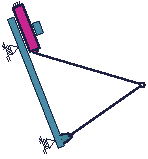
\includegraphics[width=0.32\textwidth]{part2/manovellismi/FIG/capsulismo.pdf}
     \end{center}
\begin{picture}(0,0)(0,0)
	\scriptsize{
\put(118,81){$C$}
\put(29,97){$B$}
\put(59,35){$D$}
\put(-3,90){$A$}
\put(-5,92){\rotatebox{-159}{$\longrightarrow$}}
\put(-3,80){$\infty$}
}
\end{picture}
\vskip -5.3mm
        \caption{\em Manovellismo ordinario centrato a glifo mobile.}
     \label{fig:capsulismo}
\end{wrapfigure}

\noindent a quello di figura \ref{fig:quad_D_infinito_man} mandando all'infinito
la cerniera $A$ anzich\'e la $D$.
\noindent Per dare un po' di vitalit\`a a questa nota, 
scegliamo in questo caso di rendere mobile il glifo e tenere ferma
la cerniera $B$.
Il dispositivo pratico che ne risulta \`e piuttosto
diverso nei due frangenti.
Nella stragrande maggioranza dei casi,
il manovellismo ordinario centrato viene progettato e realizzato
tenendo fisso il glifo.
Nell'altro caso si ottiene invece il
sistema articolato che \cite{sesini1} riporta a pag. 107, Fig. IV-4 (e che
noi riportiamo in figura \ref{fig:capsulismo}), 
dichiarando che ``tale meccanismo non trova notevoli applicazioni''; anche
all'autore
non risultano applicazioni rilevanti di questo
manovellismo, neppure ai nostri giorni. La figura riportata su queste note
appare per\`o piuttosto diversa
da quella che si trova in \cite{sesini1}. Questo perch\'e
abbiamo preferito privilegiare, in questo caso, la coerenza con la precedente
figura \ref{fig:quad_D_infinito}, mantenendo perci\`o gli stessi rapporti
dimensionali tra i membri del quadrilatero e gli stessi orientamenti
relativi,
piuttosto che garantire alla manovella $CD$ di potere compiere intere
rotazioni.}.
\noindent Il percorso della cerniera $C$ diventa il segmento $\sigma$,
che pu\`o essere una scanalatura (glifo) in cui scorre un cursore di forma
opportuna. Ad esempio, nei motori endotermici, i cilindri costituiscono i
glifi e gli stantuffi hanno la funzione di cursore. \`E per\`o chiaro che l'elemento che funge
da guida cava pu\`o essere invertito con l'elemento che funge da cursore,
trasformando quest'ultimo in un glifo, e
questa opportunit\`a si presenta per tutti i manovellismi, ordinari e non.
\noindent In ambito industriale il manovellismo si studia
e si progetta, come \`e ovvio, tramite l'ausilio dei programmi di calcolo 
per l'analisi di sistemi articolati.
\noindent Tuttavia il manovellismo ordinario centrato \`e talmente diffuso,
specialmente in ambito {\em automotive} (ogni vettura  a combustione
interna ne ospita in media quattro) e gli
studi che lo hanno riguardato all'inizio del secolo scorso sono cos\`i rilevanti
e fecondi di risultati, da imporre alla coscienza 
di chi insegna Meccanica Applicata l'esposizione, magari in breve,
di quella che si pu\`o chiamare ``trattazione analitica del manovellismo'';
e cos\`i faremo noi.
\begin{figure}[hbt]
     \begin{center}
     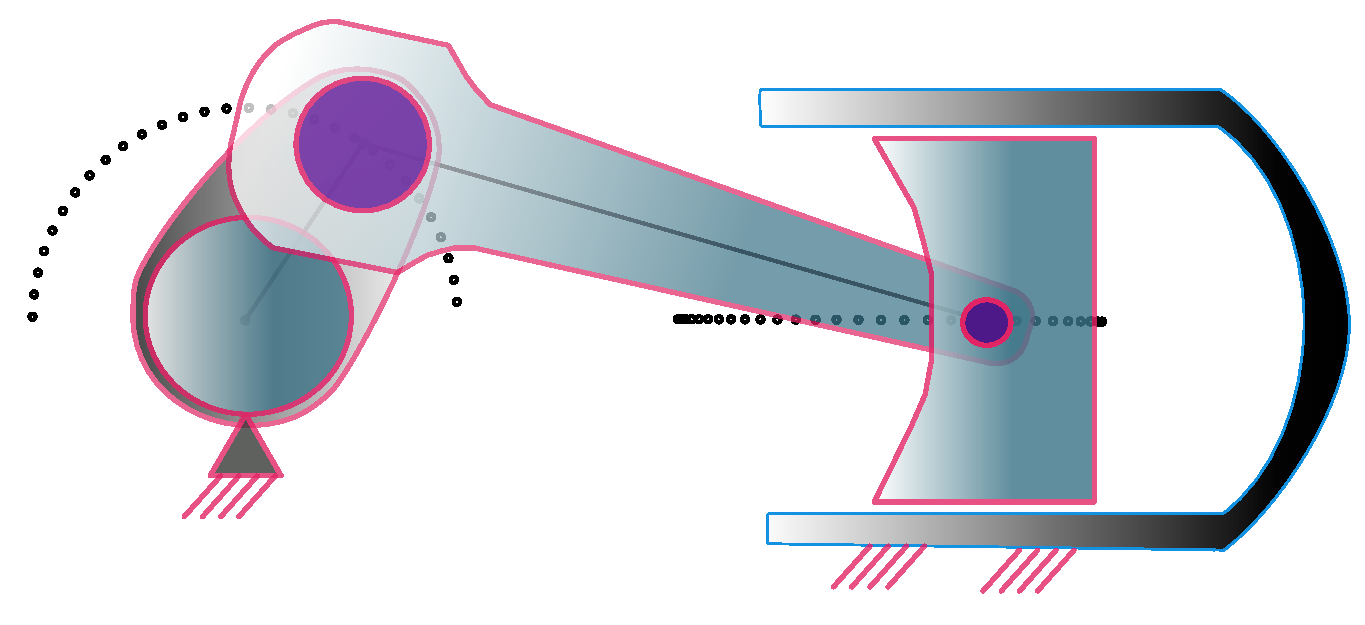
\includegraphics[width=0.85\textwidth]{part2/manovellismi/FIG/man_ord.pdf}
\begin{picture}(0,0)(270,-3)
        \scriptsize{
        \put(38,109){$B$}
        \put(53.4,74.3){$\alpha$}
        \put(187,57){$C$}
        \put(5,59){$A$}
\put(44,66.6){\line(1,0){50}}
        \put(50,73.6){\rotatebox{-67}{$\curvearrowleft$}}
}
\end{picture}
\vskip -1mm
        \caption{\em Manovellismo ordinario centrato.}
     \label{fig:man_ord}
	\end{center}
\vskip -3mm
\end{figure}
\noindent Cominciamo col dare uno sguardo al moto del {\em piede di biella}\index{piede di biella} $C$, senza pretese di esattezza, giusto per renderci conto in modo 
qualitativo del suo movimento alternativo. Riportiamo a tal fine
di nuovo il manovellismo di figura
\ref{fig:quad_D_infinito_man} nella nuova figura
\ref{fig:man_ord},
e le quantit\`a cinematiche del punto $C$, ottenute da un'analisi
numerica, in figura
\ref{fig:vel_manovellismo_ordinario_centrato}.
\begin{figure}[hbt]
\begin{center}
    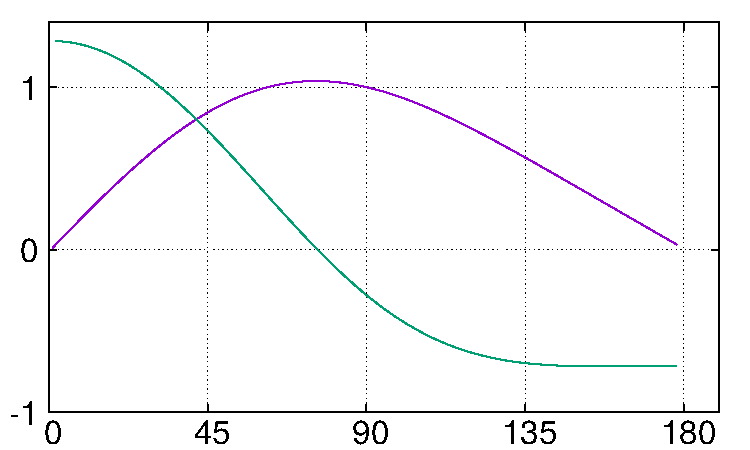
\includegraphics[width=0.55\textwidth]{part2/manovellismi/FIG/manovellismi/vel_manovellismo.pdf}
\begin{picture}(0,0)(170,25)
        \scriptsize{
        \put(80,118){$v_{\scriptscriptstyle C}$}
        \put(120,50){$a_{ \scriptscriptstyle C}$}
        \put(165,25){$\alpha$}
}
\end{picture}
        \caption{\em Velocit\`a e accelerazione nel manovellismo ordinario centrato.}
     \label{fig:vel_manovellismo_ordinario_centrato}
\end{center}
\vskip -3mm
\end{figure}
\noindent  In figura \ref{fig:man_ord}
si possono vedere le tracce
del {\em bottone di manovella}\index{bottone di manovella} $B$
e del piede di biella $C$,
mentre in figura  \ref{fig:vel_manovellismo_ordinario_centrato} sono riportati
i grafici di velocit\`a e accelerazione del punto $C$,
assumendo per la  velocit\`a angolare della manovella $AB$, di
lunghezza unitaria,
$\omega_{\scriptscriptstyle AB}=1$.
Notiamo subito, sia esaminando le tracce del piede di biella,
sia dal grafico della velocit\`a, che il punto $C$ deve rallentare 
nei punti morti (manovella con $\alpha=0$ e $\alpha=180$) fino a
fermarsi: presupposto ovvio affinch\'e il moto di $C$ si possa invertire.

\section{Espressioni Analitiche di Velocit\`a e Accelerazione del Piede
di Biella}

\noindent Con riferimento alla figura \ref{fig:moc_schematico} possiamo
innanzitutto considerare che la distanza $\overline{AC}$ \`e pari a

\begin{equation}
\overline{AC} = r \cos (\alpha) + l \cos (\beta)\,.
\end{equation}

\begin{wrapfigure}{r}{0.5\textwidth}
     \begin{center}
     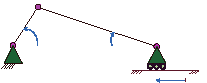
\includegraphics[width=0.48\textwidth]{part2/manovellismi/FIG/moc_schematico.pdf}
     \end{center}
\begin{picture}(0,0)(32,3)
	\scriptsize{
        \put(64,97){$B$}
        \put(68,64){$\alpha$}
        \put(54,80){$r$}
        \put(120,78){$l$}
        \put(122,64){$\beta$}
        \put(164,65){$C$}
        \put(168,24){$x$}
        \put(168,16){$\dot x$}
        \put(168,8){$\ddot x$}
        \put(34,59){$A$}
\put(54,60){\line(1,0){30}}
\put(115,60){\line(1,0){40}}
}
\end{picture}
\vskip -3.95mm
        \caption{\em Rappresentazione schematica del manovellismo ordinario centrato.}
     \label{fig:moc_schematico}
\end{wrapfigure}

\noindent \`E facile perci\`o scrivere per la coordinata $x$, che indica lo
spostamento del piede di biella ($C$) dal punto morto esterno, 
\begin{equation}
x= r+l - r \cos (\alpha) - l \cos (\beta)\,.
\label{eq:formula_manovellismo}
\end{equation}
\noindent \`E opportuno (e tradizionale) introdurre a questo punto un parametro
che caratterizza fortemente il manovellismo: si tratta del rapporto tra il raggio
di manovella e la lunghezza della biella:
\begin{equation}
\lambda= \frac{r}{l}\,.
\end{equation}
\noindent Bench\'e questo rapporto possa, in teoria, spaziare in un intervallo
amplissimo, esso \`e soggetto a restrizioni quando si desidera una manovella 
libera di compiere intere rotazioni. In tal caso $\lambda< 0.28$\footnote
{Valore di lambda per i manovellismi del motore {\em Alfa Romeo} 1600 cc della
{\em Giulia GTA Sprint}.}\footnote{Al di l\`a degli ovvi problemi che 
nascerebbero aumentando $\lambda$, problemi principalmente dovuti 
alle possibili interferenze tra organi in moto alterno, di solito gli stantuffi,
il rapporto $\lambda$ si tiene comunque piuttosto distante dal limite teorico
$\lambda=0.5$, cio\`e da quello che vedrebbe la biella di lunghezza doppia
della manovella e che consentirebbe la completa rotazione di quest'ultima.
Dalla figura \ref{fig:moc_schematico} risulta $\lambda={\sin
\beta_{\scriptscriptstyle{(\alpha= 90^{\circ})}}}$. Pertanto, nelle posizioni
$\alpha=90^{\circ}$ e $\alpha=270^{\circ}$ le forze che agiscono sullo stantuffo
solleciteranno la biella
moltiplicate per $\frac{1}{\cos \beta_{\scriptscriptstyle {\rm max}}}=\frac{1}{\sqrt{1-\lambda^2}}$; \`e evidente che valori
elevati di $\lambda$ renderebbero
la trasmissione del moto inefficiente, dando luogo a ingenti spinte laterali sul glifo
e pregiudicando dal punto di vista strutturale
gli organi meccanici coinvolti.}
risulta essere un limite ragionevole per i manovellismi ordinari centrati impiegati nei motori a combustione interna e nei compressori.
Tale limitazione non vale per manovellismi dove la manovella si comporta in
realt\`a da bilanciere, come accade nella maggior parte delle presse a
ginocchiera, dove $\lambda$ pu\`o persino superare l'unit\`a.
Osserviamo che $r \sin \alpha = l \sin\beta$, e che
$\cos \beta=\sqrt{1-\lambda^2 \sin^2\alpha}$.
Tramite queste relazioni la \ref{eq:formula_manovellismo} diventa 
\begin{equation}
x= r[1 - \cos \alpha + \frac{1}{\lambda} (1 -  \sqrt{1-\lambda^2 \sin^2\alpha})]\,.
\label{eq:formula_manovellismo_1}
\end{equation}
\noindent Derivare rispetto al tempo una prima, quindi una seconda volta
la \ref{eq:formula_manovellismo_1},
allo scopo di ottenere velocit\`a e accelerazione del piede di biella,
non presenta certo difficolt\`a. Tale calcolo per\`o somiglierebbe
a un esercizio
meramente didattico di studio ``a livello liceale'' delle operazioni di
derivazione di semplici funzioni.
Come \`e noto, infatti, le derivate di radicali portano radicali, e 
le funzioni $\dot x$ e $\ddot x$, ottenute per questa via, dovrebbero
essere graficate con grande sforzo di calcolo,
oppure per via numerica, circostanza quest'ultima che vanificherebbe lo spirito
di questo percorso.


\noindent Si preferisce pertanto partire da una formula pi\`u semplice,
che approssimi lo spostamento del piede di biella, e ricavare da
quest'ultima le quantit\`a cinematiche derivate.
La strada \`e quella di esprimere il radicando della \ref{eq:formula_manovellismo_1} tramite i primi due termini del suo sviluppo in
serie, sviluppo eseguito considerando $\lambda$
(e non gi\`a $\alpha$) come variabile indipendente:
\begin{equation}
\sqrt{1-\lambda^2 \sin^2\alpha}\simeq 1 - \frac{1}{2} \lambda^2\sin^2\alpha \,.\notag
%\label{eq:svil_sqrt}
\end{equation}
\noindent Otteniamo cos\`i l'espressione arrestata al secondo ordine per lo
spostamento del piede di biella,
che risulter\`a tanto pi\`u  approssimato quanto pi\`u piccolo sar\`a
il rapporto $\lambda$:
\begin{equation}
x= r[1 - \cos \alpha + \frac{1}{2} \lambda \sin^2\alpha]\,;
\label{eq:formula_manovellismo_approx0}
\end{equation}
\noindent essendo poi
\begin{equation}
\sin^2\alpha= \frac{1 - \cos 2\alpha}{2}\,,
\label{eq:formula_manovellismo_approx}
\end{equation}
\noindent otteniamo finalmente   
\begin{equation}
x= r[1 +\frac{\lambda}{4} - \cos \alpha - \frac{\lambda}{4} \cos 2\alpha]\,.
\label{eq:formula_manovellismo_approx_1}
\end{equation}
\noindent La velocit\`a ``approssimata al second'ordine'' si
trova derivando rispetto al tempo la \ref{eq:formula_manovellismo_approx_1},
tenendo presente che ${\rm d}\alpha/{\rm d}t=\omega$:
\begin{equation}
\dot x= r\omega[\sin \alpha +\frac{\lambda}{2} \sin 2\alpha]\,,
\label{eq:formula_manovellismo_approx_vel}
\end{equation}
\noindent mentre per l'accelerazione avremo
\begin{equation}
\ddot x= r\omega^2[\cos \alpha +\lambda \cos 2\alpha]\,.
\label{eq:formula_manovellismo_approx_acc}
\end{equation}
\noindent Le espressioni \ref{eq:formula_manovellismo_approx_vel} e \ref{eq:formula_manovellismo_approx_acc}
mostrano chiaramente un andamento delle due grandezze cinematiche
composto da due armoniche.


\noindent Tramite le seguenti due osservazioni,
proviamo a evidenziare il lato a nostro avviso
pi\`u significativo
di questo studio analitico del manovellismo ordinario.
In primo luogo notiamo che per $\lambda$ molto
piccoli (biella molto lunga in rapporto al raggio di manovella), il moto del
piede di biella risulta coincidere sostanzialmente col moto
armonico:
\begin{equation}
\begin{split}
r-x=r\cos \alpha\,,\;\;\; \dot x=\omega r \sin\alpha\,\;\; {\rm e}\;\;\;\ddot x= \omega^2 r \cos\alpha\,. 
\end{split}
\label{eq:formule_primo_o}
\end{equation}
\begin{wrapfigure}{r}{0.5\textwidth}
     \begin{center}
     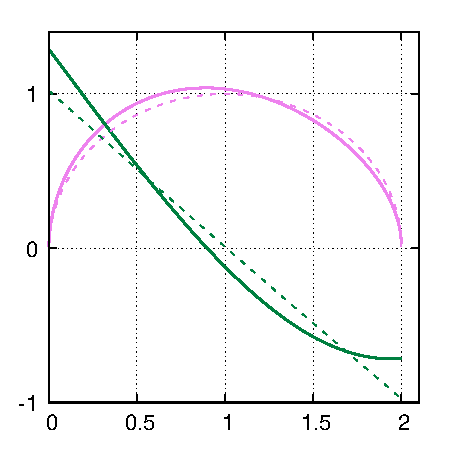
\includegraphics[width=0.48\textwidth]{part2/manovellismi/FIG/manovellismi/vel_manovellismo_x.pdf}
     \end{center}
\begin{picture}(0,0)(0,0)
	\scriptsize{
	\put(66,100){${\ddot x}(x)$}
	\put(80,168.5){${\dot x}(x)$}
}
\end{picture}
\vskip -5mm
        \caption{\em Velocit\`a e accelerazione del piede di biella in funzione del suo spostamento normalizzato per $r$ ($1^o$ ordine tratteggiato).}
     \label{fig:vel_manovellismo_x}
\end{wrapfigure}

\noindent \`E interessante esprimere
velocit\`a e accelerazione del piede di biella 
in funzione della coordinata $x$
anzich\'e dell'angolo $\alpha$, figura \ref{fig:vel_manovellismo_x}.
In tal caso, posto $\omega = 1$, quadrando e sommando membro a membro le formule che esprimono
velocit\`a e spostamento approssimati al primo ordine abbiamo
\begin{equation}
(r-x)^2 + {\dot x}^2=r^2\,.
\label{eq:cerchio_vel}
\end{equation}
\noindent La \ref{eq:cerchio_vel} rappresenta l'equazione di una circonferenza
di raggio $r$ e centrata a una distanza $r$ dal punto morto esterno: tale
risulter\`a quindi  l'andamento della
velocit\`a, graficata prendendo $x/r$ come ascissa.
Questo andamento verr\`a ovviamente modificato 
da valori di 
$\lambda$ non  trascurabili, quando cio\`e il moto del piede di 
biella si scoster\`a sensibilmente dal moto armonico.
La figura \ref{fig:vel_manovellismo_x} mostra l'andamento effettivo di
$\dot x(x)$, che tiene conto anche delle successive armoniche,
per $\lambda=0.28$.

\noindent La seconda osservazione riguarda l'accelerazione.
Il grafico di $\ddot x(x)$ \`e anch'esso riportato nella figura appena
citata e ha una forma che somiglia a quella di una parabola.
Fermandoci per\`o al primo ordine,
tale grafico sarebbe una retta. Infatti dalle \ref{eq:formule_primo_o}
otteniamo subito $\cos \alpha=(r-x)/r$ e poi $\ddot x = \omega^2(r-x)$.
Ponendo quindi come al solito $\omega=1$, il grafico di $\ddot x(x)$ sar\`a
una retta a quarantacinque gradi, passante dallo zero a distanza $r$ dal
punto morto esterno. In prima approssimazione, possiamo pertanto
attribuire al piede di biella una accelerazione che varia linearmente
tra i due punti morti: considerazione questa che porta con s\'e una decisa
facilit\`a di calcolo.
Un'ultima osservazione riguarda la possibilit\`a di calcolare
i due valori di accelerazione nei punti morti tramite la formula 
\ref{eq:formula_manovellismo_approx_acc}: otteniamo
$\ddot x(0^{\circ})= \ddot x(0)=r \omega^2(1+\lambda)$  e
$\ddot x(180^{\circ})= \ddot x(2r)=r \omega^2(1-\lambda)$. Lasciamo al 
paziente e volenteroso lettore il compito di mostrare che 
questi due valori
dell'accelerazione del piede di biella nei punti morti sono esatti:
essi non
risentono cio\`e dell'approssimazione introdotta nello spostamento dalla
\ref{eq:formula_manovellismo_approx_1}.

\section{Velocit\`a e Accelerazione del Piede di Biella: Analisi
mediante i Moti Relativi}

\noindent Come nello studio del quadrilatero, \`e possibile, anche in questo caso,
esprimere le quantit\`a cinematiche dei diversi punti del manovellismo
mediante le relazioni che legano queste grandezze quando
si considerano i moti relativi che avvengono tra i vari membri.

\begin{wrapfigure}{r}{0.5\textwidth}
     \begin{center}
     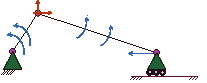
\includegraphics[width=0.48\textwidth]{part2/manovellismi/FIG/moc_schematico_graf.pdf}
     \end{center}
\begin{picture}(0,0)(32,7)
	\scriptsize{
        \put(58,94){$B$}
        \put(43,85){${\omega_{\scalebox{.5}{AB}}}$}
        \put(55,51){${\dot\omega_{\scalebox{.5}{AB}}}$}
        \put(102,91){${\omega_{\scalebox{.5}{BC}}}$}
        \put(124,84){${\dot\omega_{\scalebox{.5}{BC}}}$}
        \put(136,58){${{\bm v}_{\scalebox{.5}{C}}}$}
        \put(164,65){$C$}
        \put(34,59){$A$}
}
\end{picture}
\vskip -4mm
        \caption{\em Velocit\`a e accelerazioni nei moti relativi del manovellismo.}
     \label{fig:moc_schematico_graf}
\end{wrapfigure}

\noindent Con riferimento alla figura \ref{fig:moc_schematico_graf},
posizioniamo un sistema di riferimento traslante centrato nel
{\em bottone di manovella}\index{bottone di manovella} $B$. 
Possiamo cos\`i esprimere la velocit\`a del piede di biella come somma delle
due componenti:
quella relativa
e quella di trascinamento
\begin{equation}
{{\bm v}_{\scriptscriptstyle{C}}}= 
{{\bm v}_{\scriptscriptstyle{C}}}_{\scriptscriptstyle{{\rm rel}}}+
{{\bm v}_{\scriptscriptstyle{B}}}\,,
\label{eq:man_vel_graf0}
\end{equation}
\noindent ovvero esprimendo i due addendi di destra tramite le loro relazioni con
le velocit\`a angolari di biella e manovella,
\begin{equation}
{{\bm v}_{\scriptscriptstyle{C}}}= 
{\omega_{\scriptscriptstyle{BC}}}|\overrightarrow{BC}|\widehat{{\perp{BC}}}+
{{\bm v}_{\scriptscriptstyle{B}}}\,.
\label{eq:man_vel_graf1}
\end{equation}
\noindent La \ref{eq:man_vel_graf1} \`e un'equazione vettoriale nella quale
la direzione di tutti e tre i termini \`e nota
mentre $|{{\bm v}_{\scriptscriptstyle{C}}}|$ e 
${\omega_{\scriptscriptstyle{BC}}}$ risulteranno incogniti, supponendo data
la velocit\`a angolare della manovella. Si ripropone quindi
lo schema risolutivo illustrato in figura \ref{fig:f116},
dal quale ricaveremo
il valore della velocit\`a del piede di biella e la velocit\`a angolare
della biella.
Per quanto riguarda le accelerazioni possiamo scrivere
\begin{equation}
{{\bm a}_{\scriptscriptstyle{C}}}= 
{{\bm a}_{\scriptscriptstyle{C}}}_{\scriptscriptstyle{{\rm rel}}}+ 
{{\bm a}_{\scriptscriptstyle{B}}}\,. 
\label{eq:acc_man_graf0}
\end{equation}
\noindent Come abbiamo gi\`a chiarito altrove, conviene scrivere il termine
${{\bm a}_{\scriptscriptstyle{C}}}_{\scriptscriptstyle{{\rm rel}}}$
 come somma delle sue due
componenti: quella avente direzione parallela alla biella e diretta verso $B$
(componente normale) e quella ortogonale alla biella stessa.
Anche il termine ${{\bm a}_{\scriptscriptstyle{B}}}$ si pu\`o scrivere 
mediante la somma delle sue componenti,
quella radiale e quella tangenziale, le quali
risulteranno note
supponendo di conoscere la velocit\`a e la accelerazione angolari della
manovella.  Otteniamo in questo modo
\begin{equation}
{{\bm a}_{\scriptscriptstyle{C}}}= 
-{\omega_{\scriptscriptstyle{BC}}}^2 \overrightarrow{BC}+
{\dot\omega_{\scriptscriptstyle{BC}}}|\overrightarrow{BC}|\widehat{{\perp{BC}}}
-{\omega_{\scriptscriptstyle{AB}}}^2 \overrightarrow{AB}+
{\dot\omega_{\scriptscriptstyle{AB}}}|\overrightarrow{AB}|\widehat{{\perp{AB}}}\,.
\label{eq:acc_man_graf1}
\end{equation}
\noindent Ancora una volta siamo di fronte a una equazione vettoriale
dove le incognite sono
il modulo dell'accelerazione del piede di biella
$|{{\bm a}_{\scriptscriptstyle{C}}}|$ e l'accelerazione angolare della biella
${\dot\omega_{\scriptscriptstyle{BC}}}$, essendo note le direzioni di
tutti i vettori.
Una possibile soluzione \`e quindi, anche qui, 
lo schema grafico di figura \ref{fig:f116}; per inciso, la \ref{eq:acc_man_graf1} \`e formalmente identica alla \ref{eq:e_a_quad_schematico2},
la qual cosa non ci stupisce visto che stiamo di nuovo trattando
la cinematica di un quadrilatero, sia pure degenere.
Riteniamo di dover ribadire che il ruolo dei termini noti
e di quelli incogniti possono essere scambiati a discrezione: se considerassimo
assegnate la velocit\`a e l'accelerazione del piede di biella potremmo ricavare,
dalle \ref{eq:man_vel_graf1} e \ref{eq:acc_man_graf1},
le quantit\`a {${\omega_{\scalebox{.5}{AB}}}$} e
{${\dot\omega_{\scalebox{.5}{AB}}}$} della manovella $AB$.

\section{Manovellismi Non Ordinari}

\noindent Come \`e stato accennato nel paragrafo introduttivo, se ad andare
all'infinito \`e una delle due cerniere mobili di un quadrilatero si ottengono,
sostituendo opportunamente le aste e le cerniere degeneri con
membri appropriati,
i {\em manovellismi non ordinari}\index{manovellismo!non ordinario}. Questi manovellismi, ovviamente {\em cinematicamente
equivalenti}\index{equivalenza cinematica} ai quadrilateri degeneri che li 
originano,
vengono spessissimo chiamati, con ragione,
meccanismi 
{\em a glifo rotante}\index{glifo!rotante} ovvero
{\em a glifo oscillante}\index{glifo!oscillante},
dando per scontato che un preciso membro di tali meccanismi
sia un glifo. Non ci stanchiamo
di ripetere che, a rigore, i due membri dell'accoppiamento glifo-cursore
possono sempre essere scambiati tra loro senza alcuna mutazione
della cinematica del sistema.
Prima di entrare nel vivo di questo paragrafo, desideriamo esporre una breve
precisazione, che per la verit\`a avrebbe potuto precedere anche la
trattazione dei manovellismi ordinari, ma che si rende ancora
pi\`u necessaria in questa sede: cosa
intendiamo, esattamente, con la locuzione
{\em equivalenza cinematica}\index{equivalenza
cinematica}? Ancora pi\`u esplicitamente, quando asseriamo che la cerniera
$D$ e il bilanciere $DC$ del quadrilatero
degenere di figura \ref{fig:quad_D_infinito_man} vengono sostituiti
dalla coppia glifo-cursore $\sigma$, ottenendo in tal modo il
manovellismo ordinario
equivalente, di quale equivalenza parliamo?
Nello studio dei manovellismi si parla di meccanismo equivalente
quando la biella (o un corpo che la sostituisce) sar\`a interessata dallo
stesso moto piano, mantenendo per tutti i punti di biella le stesse
traiettorie, le stesse velocit\`a e le stesse accelerazioni. Nel
caso che abbiamo studiato dei manovellismi ordinari l'equivalenza
del comportamento della biella di figura \ref{fig:quad_D_infinito_man} con
la cerniera $D$ a grande distanza o con la coppia glifo-cursore $\sigma$ 
sembra all'autore sufficientemente evidente.
Qualche attenzione in pi\`u \`e richiesta
nello studio dei manovellismi non ordinari.

\noindent Giusto per fissare qualche idea circa il comportamento di 
un quadrilatero che degenera tramite l'allontanamento di una delle
due cerniere (perfettamente equivalenti) $B$ oppure $C$, eseguiamo un tentativo
di analisi qualitativa tramite i nostri consueti (e rudimentali)
strumenti di indagine numerica.
\begin{figure}[hbt]
\centering
\begin{minipage}[b]{0.52\textwidth}
\centering
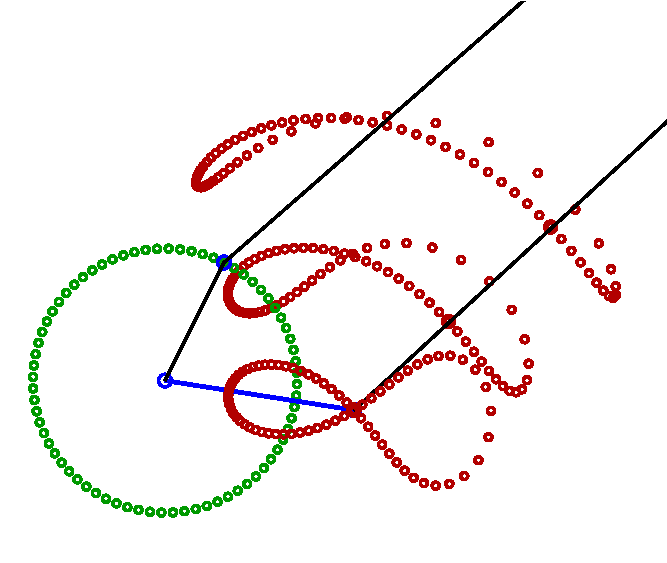
\includegraphics[width=0.9\textwidth]{part2/manovellismi/FIG/manovellismi/c_infinito.pdf}
\begin{picture}(0,0)(138,-6)
\scriptsize{
\put(11,65){$B$}
\put(110,107){$C$}
\put(110,100){\rotatebox{42.45}{$\longrightarrow$}}
\put(113,98){$\infty$}
\put(2,32){$A$}
\put(50,23){$D$}
\put(52.5,37.5){$\alpha$}
\put(78,60){$\beta$}
\put(101,71){$\gamma$}
\color{red}
\put(99.3,83.3){\rotatebox{-47.55}{\line(1,0){15}}}
\put(73,60){\rotatebox{-47.55}{\line(1,0){15}}}
\put(48,38){\rotatebox{-47.55}{\line(1,0){15}}}
}
\end{picture}
      \caption{\em Quadrilatero degenere ottenuto mandando la cerniera $C$ a distanza infinita.}
 \label{fig:c_infinito}
\end{minipage}\hfill\hfill
\begin{minipage}[b]{0.40\textwidth}
\centering
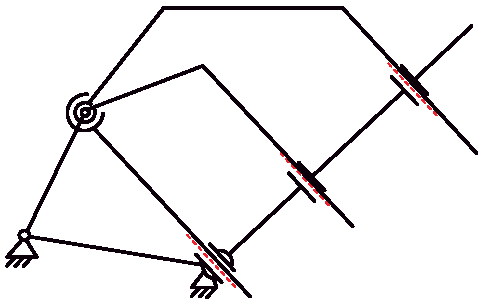
\includegraphics[width=0.9\textwidth]{part2/manovellismi/FIG/glifi_c_infinito.pdf}
\vspace*{10mm}
\begin{picture}(0,0)(139,18)
\scriptsize{
\put(13,65){$B$}
\put(110,107){$C$}
\put(110,100){\rotatebox{42.45}{$\longrightarrow$}}
\put(113,98){$\infty$}
\put(0,32){$A$}
\put(54,14){$D$}
\put(50,44){$a)$}
\put(74,65){$b)$}
\put(100,91){$c)$}
}
\end{picture}
      \caption{\em Possibili meccanismi a glifo mobile derivati dalla figura a lato.}
     \label{fig:glifi_c_infinito}
\end{minipage}
\end{figure}
\noindent Abbiamo scelto, con criterio del tutto arbitrario, di rendere
improprio l'asse della cerniera $C$. Come nel caso dei manovellismi ordinari,
la scelta della direzione secondo la quale mandare tale cerniera 
a grande distanza non
\`e indifferente. Quando la cerniera, come in questo caso, \`e mobile
 tale direzione muta durante il 
movimento del meccanismo. Notiamo per\`o che, scelta in un dato istante
la direzione del punto improprio $C$, essa rimarr\`a, durante il movimento,
costante rispetto alla direzione del segmento $BD$;
in altre parole l'angolo tra la direzione del punto improprio
e $BD$ si manterr\`a costante.
Ci\`o accade in quanto il triangolo $\triangle{BCD}$ presenta angolo costante
e nullo in $C$. Ritenendo quindi le lunghezze dei lati
$BC$ e $CD$ costanti, anche se infinite, rimarranno invariati durante
il movimento anche gli altri suoi angoli\footnote
{
La lunghezza del lato $BD$, ovviamente, non si mantiene costante. Essa
per\`o risulta infinitesimale rispetto alle lunghezze degli altri
due lati, pertanto la sua variazione provoca alterazioni infinitesimali
e trascurabili del triangolo $\triangle{BCD}$.
}.
Nel caso delle figure \ref{fig:c_infinito} e \ref{fig:glifi_c_infinito}
la direzione scelta coincide con la perpendicolare al segmento $BD$,
scelta che consente di ottenere {\em manovellismi non ordinari
centrati}\index{manovellismo!non ordinario}.
\noindent In figura \ref{fig:c_infinito} sono riportate tre curve di biella
relative a tre punti che giacciono sul membro $DC$.
Lo scopo di tale figura \`e quello 
di rendere maggiormente evidente il moto del piano di
biella nei pressi del bilanciere  ``improprio''.
Da questa analisi si pu\`o notare che nei punti di intersezione con 
il bilanciere $DC$, le curve di biella sono 
ortogonali ad esso. La figura, rimarcando questa circostanza, facilita
l'intuizione. Tali direzioni
erano peraltro prevedibili a valle di semplici ragionamenti geometrici, osservando che 
tutti i punti di biella che giacciono su $DC$ descrivono, nel loro
moto relativo a tale membro,  delle circonferenze di centro $C$,
le cui tracce sono in figura rappresentate da brevi segmenti:
$\alpha$, $\beta$ e $\gamma$.
La condizione poi che il punto $C$ si trovi a grande distanza ci
autorizza, come abbiamo appena sopra chiarito, a ritenere costante
l'angolo compreso tra $DC$ e il segmento $DB$,
pari nel nostro caso a $90^{\circ}$. 
Queste considerazioni ci consentono di sostituire la cerniera in $C$ con
gli accoppiamenti prismatici che danno origine alla figura
\ref{fig:glifi_c_infinito}.
\noindent I tre meccanismi a), b) e c) sono, da un punto
di vista cinematico, un solo meccanismo, essendo il piano di biella lo stesso
per le tre soluzioni e rendendo ridondante la distinzione della cerniera
in $B$ in tre cerniere separate.
I tre sistemi articolati   
presentano un glifo sul bilanciere $CD$ dove scorre la relativa biella.
Oltre a ripetere (lo abbiamo detto gi\`a troppe volte) che il ruolo
di chi porta la
scanalatura (glifo) e di chi invece fa da cursore possono indifferentemente
essere scambiati, osserviamo che tali
accoppiamenti prismatici possono essere dislocati in qualsiasi punto della
biella equivalente. 
\noindent In particolare, considerando il meccanismo a) di figura \ref{fig:glifi_c_infinito}, che riteniamo maggiormente significativo,
possiamo ottenere i sistemi articolati equivalenti
 di figura \ref{fig:c_infinito_equivalenti}.

\begin{figure}[hbt]
\centering
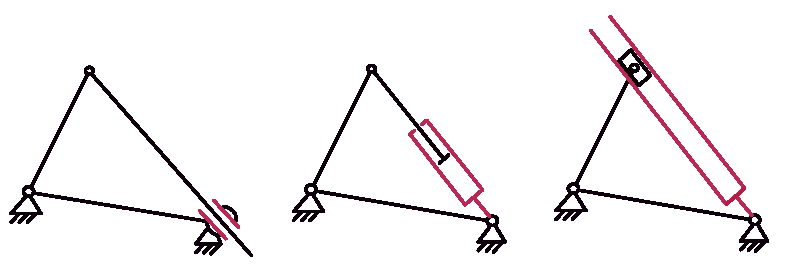
\includegraphics[width=0.9\textwidth]{part2/manovellismi/FIG/c_infinito_equivalenti.pdf}
\begin{picture}(0,0)(320,0)
\scriptsize{
\put(46,75){\tiny biella equivalente}
\put(45,75){\rotatebox{220}{$\longrightarrow$}}
\put(161,75){\tiny biella equivalente}
\put(159,75){\rotatebox{220}{$\longrightarrow$}}
\put(268,86){\tiny biella equivalente}
\put(254,85){\rotatebox{180}{$\longrightarrow$}}
\put(94,14){\tiny glifo}
\put(90,22){\rotatebox{180}{$\longrightarrow$}}
\put(146,45){\tiny glifo}
\put(156,41){\rotatebox{0}{$\longrightarrow$}}
\put(253,45){\tiny glifo}
\put(264,41){\rotatebox{0}{$\longrightarrow$}}
\put(0,50){$1)$}
\put(113,50){$2)$}
\put(222,50){$3)$}
}
\end{picture}
      \caption{\em Manovellismi non ordinari centrati equivalenti.}
 \label{fig:c_infinito_equivalenti}
\end{figure}

\noindent I tre meccanismi qui riportati presentano glifi
oscillanti attorno alla cerniera $D$, dove essi sono incernierati.
La lunghezza della ``biella'' \`e, dalla configurazione $1)$ alla
configurazione $3)$,  via via decrescente fino ad annullarsi.
Nel meccanismo $3)$ il piano di biella con tutte le sue curve
va pensato infatti solidale al cursore che scorre nel glifo.
Occorre per\`o precisare che, quando si parla di glifi oscillanti e ci si riferisce
appunto alla figura \ref{fig:c_infinito_equivalenti}, caso $3)$, ancora
pi\`u delle curve
dei punti di biella interessa il movimento del glifo stesso,
il quale \`e un bilanciere, e come tale si muove.

\section{Meccanismo a Ritorno Rapido}\index{meccanismo a ritorno rapido}\index{guida di Fairbairn}

La figura \ref{fig:c_infinito_quick} riporta nuovamente il meccanismo
di figura \ref{fig:c_infinito_equivalenti}, caso $3)$, ruotato
di un angolo opportuno, in modo da porre il suo telaio in verticale. 
\begin{figure}[hbt]
\centering
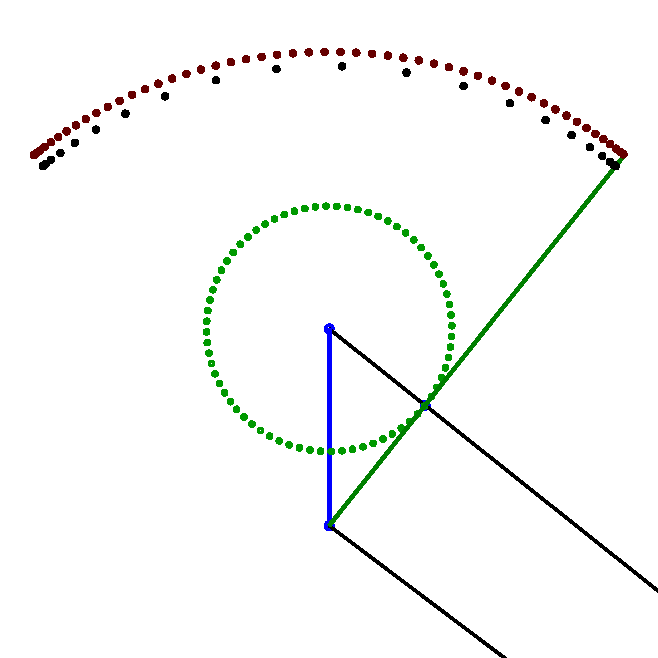
\includegraphics[width=0.9\textwidth]{part2/manovellismi/FIG/manovellismi/c_infinito_quick.pdf}
\begin{picture}(0,0)(250,0)
\scriptsize{
\put(235,245){$V$}
\put(136,125){$B$}
\put(73,158){$A$}
\put(73,62){$D$}
\put(180,50){$C$}
\put(175,50){\rotatebox{-42}{$\longrightarrow$}}
\put(173,40){$\infty$}
}
\end{picture}
      \caption{\em Meccanismo a ritorno rapido.}
 \label{fig:c_infinito_quick}
\end{figure}
\noindent A una rotazione completa della manovella
$AB$, di solito a velocit\`a $\omega$ costante, corrispondono
un'oscillazione di andata del glifo e una di ritorno che si svolgono
impiegando tempi diversi fra loro. In particolare, come abbiamo gi\`a 
visto nello studio dei quadrilateri, pagina
\pageref{eq:angoli_andata_ritorno}, tali tempi
saranno proporzionali ai rispettivi angoli di manovella.
Nella figura poc'anzi citata, ottenuta da un'analisi numerica,
non trova espressione grafica il pattino
che deve permettere al punto $B$ di scorrere
in una apposita scanalatura dell'asta $DV$, che per questo
assume generalmente il nome di glifo. Con la speranza  di porre
rimedio a tale lacuna grafica, riportiamo la prossima illustrazione,
nella quale
si pu\`o anche apprezzare l'utilizzo  concreto di questo manovellismo.
\begin{figure}[hbt]
\centering
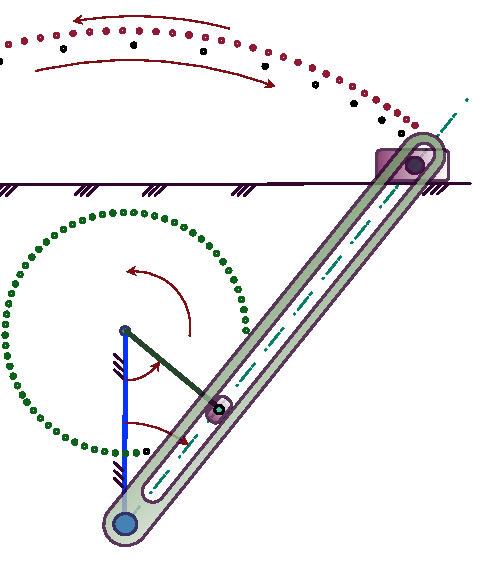
\includegraphics[width=0.9\textwidth]{part2/manovellismi/FIG/fairbairn.pdf}
\begin{picture}(0,0)(300,10)
\scriptsize{
\put(42,376){\tiny andata lenta}
\put(40,347){\tiny ritorno rapido}
\put(258,298){$V$}
\put(251,278){$K$}
\put(175,287){\tiny slitta portautensile}
\put(135,107){$B$}
\put(50,211){$\omega=cost$}
\put(66,126){$\alpha$}
\put(70,106){$\beta$}
\put(42,164){$A$}
\put(32,28){$D$}
}
\end{picture}
      \caption{\em Meccanismo di Fairbairn.}
 \label{fig:fairbairn}
\end{figure}
\noindent La {\em guida di Fairbairn}\index{glifo!di Fairbairn}\index{Fairbairn, guida di},
rappresentata in figura \ref{fig:fairbairn},
si ottiene dal meccanismo
di figura \ref{fig:c_infinito_quick} con l'aggiunta di
una bielletta (o biscottino) di
snodo oppure di un opportuno accoppiamento prismatico (\cite{sesini1}, Fig. IV-8,
pag. 108, ma anche \cite{hartog}, pag. 168) in modo tale da permettere alla
sommit\`a
del glifo di azionare una slitta rettilinea. Tale soluzione costituiva,
fra l'altro,
il cuore di una ben nota macchina utensile che necessita di una corsa di andata
``lenta'' e di un ritorno ``rapido''.
Le tracce lasciate dalla sommit\`a del glifo, durante il suo movimento, dovrebbero dare
conto, mediante la loro spaziatura, delle differenti velocit\`a di $V$ durante
un ciclo di manovella. Le stesse spaziature, proiettate in pianta, dovrebbero
altrettanto rendere l'idea della velocit\`a del punto $K$, quindi della velocit\`a
del portautensile.
Anche qui, come nel caso del manovellismo ordinario centrato, \`e possibile
impostare le equazioni che legano l'angolo $\beta$ percorso dal glifo
all'angolo $\alpha$ di manovella;
derivando queste equazioni
rispetto ad $\alpha$ oppure rispetto al tempo si otterranno infine
le equazioni della cinematica del glifo oscillante centrato. Analogamente,
non presenterebbe certo difficolt\`a alcuna mettere
 in relazione l'angolo di oscillazione del glifo con lo spostamento
della slitta portautensile, della quale si otterrebbero finalmente
 velocit\`a e accelerazione, come mostrano
importanti autori, ad esempio \cite{hartog}, pag. 168.
Non ce la sentiamo per\`o di seguirli in tale percorso,
e ci accontentiamo dell'analisi numerica
riportata in modo qualitativo nelle figure
 \ref{fig:c_infinito_quick} e
 \ref{fig:fairbairn}, mediante le tracce del bottone di manovella
 e della estremit\`a del particolare glifo che abbiamo scelto di
proporre come esempio.

\noindent A nostro parere, dalla trattazione analitica del glifo
non emergono importanti spunti didattici,
al di l\`a dei meri passaggi trigonometrici:
i volenterosi e curiosi studenti
sapranno agilmente trovare tali calcoli nella citata bibliografia, se
interessati.
Per contro, colui che si vedr\`a assegnato il compito di progettare realmente
un meccanismo a ritorno rapido si affider\`a ai contemporanei codici numerici
di simulazione di meccanismi che  forniscono, con precisione, tutte le
grandezze cinematiche in gioco.
Inoltre sottolineiamo di nuovo che
 l'importanza di questo meccanismo risiede nella 
possibilit\`a di avere tempi di andata e ritorno sensibilmente diversi fra
loro, in modo da non sprecare tempo prezioso nella fase
oziosa del moto dell'utensile,
pi\`u che nella conoscenza puntuale della velocit\`a o della
accelerazione di quest'ultimo.
Nel nostro caso, invero un po' estremo,  abbiamo $\alpha_a=257^{\circ}$ e $\alpha_r=103^{\circ}$ che permettono
al tempo di andata, corrispondente al tempo di lavoro dell'utensile, di essere
pi\`u che doppio rispetto al tempo ``morto'' del ritorno.
Ai tempi in cui le macchine utensili venivano realizzate tramite pregiate
fusioni in ghisa, il glifo di {\em Fairbairn} era l'azionamento
principale della {\em limatrice}\index{limatrice}.
A proposito di questa applicazione, sottolineiamo che
la velocit\`a massima, raggiunta dalla slitta durante
la fase di andata (lenta), si manifesta quando il punto
$K$ \`e allineato coi punti $A$, $D$ e $B$. Essa \`e facilmente calcolabile
e vale, con $K$ in tale
posizione, $|v_{max}|=|\omega| |\overrightarrow{AB}||\overrightarrow{KD}|/|\overrightarrow{BD}|$; essa
rappresenta la velocit\`a  di taglio nominale dell'utensile.

\noindent Mi si permetta (tanto  tempo \`e trascorso quindi mi sento al sicuro da
rivendicazioni o proteste di carattere commerciale) di citare la ``gloriosa
e indistruttibile'' limatrice
Garavaglia.
Tutte le officine meccaniche rispettabili
ne avevano almeno una a disposizione. L'autore per\`o confessa che, gi\`a
trent'anni or sono, queste macchine beneficiavano di
notevolissimi periodi di riposo.

\section{Cinematica del Meccanismo a Ritorno Rapido: Analisi 
mediante i Moti Relativi}

\noindent La soluzione grafica che abbiamo esposto per l'analisi cinematica
di quadrilateri e manovellismi ordinari si pu\`o naturalmente estendere
anche al caso del meccanismo a ritorno rapido.
\noindent Riferendoci alla figura \ref{fig:soluzione_grafica_glifo}
posizioniamo, in questo caso, un sistema di riferimento relativo (al quale cio\`e
verranno riferite le grandezze relative) che ruota solidalmente con il
glifo ed \`e centrato in $D$.
Siamo in grado ora di esprimere la velocit\`a del punto $B$ (bottone di
manovella) mediante la somma delle due componenti: quella relativa
e quella di trascinamento:
\begin{equation}
{{\bm v}_{\scriptscriptstyle{B}}}_{\scriptscriptstyle{{\rm ass}}}= 
{{\bm v}_{\scriptscriptstyle{B}}}_{\scriptscriptstyle{{\rm rel}}}+
{{\bm v}_{\scriptscriptstyle{B}}}_{\scriptscriptstyle{{\rm tr}}}\,,
\label{eq:glifo_vel_graf0}
\end{equation}
\noindent ovvero, 
\begin{equation}
{{\bm v}_{\scriptscriptstyle{B}}}_{\scriptscriptstyle{{\rm ass}}}= 
{{\bm v}_{\scriptscriptstyle{B}}}_{\scriptscriptstyle{{\rm rel}}}+
{\omega_{\rm g}}|\overrightarrow{DB}|\widehat{{\perp{DB}}}\,.
\label{eq:glifo_vel_graf1}
\end{equation}

\begin{wrapfigure}{r}{0.5\textwidth}
     \begin{center}
     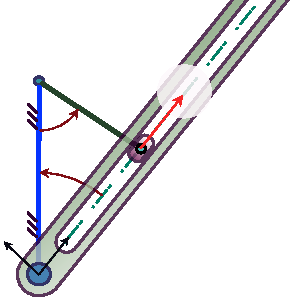
\includegraphics[width=0.48\textwidth]{part2/manovellismi/FIG/soluzione_grafica_glifo.pdf}
     \end{center}
\begin{picture}(0,0)(32,7)
	\scriptsize{
        \put(130,113){$B$}
        \put(41,37){$D$}
        \put(45,162){$A$}
        \put(34,71){$\scriptstyle{y'}$}
        \put(71,72){$\scriptstyle{x'}$}
        \put(62,130){${\omega_{\rm{m}}}$,}
        \put(77,130){${\dot\omega_{\rm{m}}}$}
        \put(63,112.5){${\omega_{\rm{g}}}$,}
        \put(78,112.5){${\dot\omega_{\rm{g}}}$}
        \put(132,157){${{\bm v}_{\scalebox{.5}{B}}}$,}
        \put(143,157){${{\bm a}_{\scalebox{.5}{B}}}$}
}
\end{picture}
\vskip -1.3mm
        \caption{\em Velocit\`a e accelerazioni nei moti relativi del meccanismo a ritorno rapido.}
     \label{fig:soluzione_grafica_glifo}
\end{wrapfigure}
\noindent La \ref{eq:man_vel_graf1} \`e un'equazione vettoriale nella quale
la direzione di tutti e tre i termini \`e nota
mentre
$|{{\bm v}_{\scriptscriptstyle{B}}}_{\scriptscriptstyle{{\rm rel}}}|$
e ${\omega_{\rm g}}$ sono incogniti, una volta data
la velocit\`a angolare della manovella. Anche qui riproponiamo quindi
lo schema risolutivo illustrato in figura \ref{fig:f116},
mediante il quale ricaveremo i valori delle incognite.

\noindent Per quanto riguarda le accelerazioni scriviamo
\begin{equation}
{{\bm a}_{\scriptscriptstyle{B}}}_{\scriptscriptstyle{{\rm ass}}}= 
{{\bm a}_{\scriptscriptstyle{B}}}_{\scriptscriptstyle{{\rm rel}}} 
+{{\bm a}_{\scriptscriptstyle{B}}}_{\scriptscriptstyle{{\rm tr}}} 
+{{\bm a}_{\scriptscriptstyle{B}}}_{\scriptscriptstyle{{\rm cor}}}\,,
\label{eq:acc_glifo_graf0}
\end{equation}
\noindent dove si nota la presenza del termine dell'accelerazione di {\em Coriolis}
dovuta alla rotazione del sistema di riferimento relativo.
Come al solito sostituiamo alle accelerazioni le loro componenti tangenziali
e normali ottenendo
\begin{equation}
{{\bm a}_{\scriptscriptstyle{B}}}_{\scriptscriptstyle{{\rm ass}}}= 
{{\bm a}_{\scriptscriptstyle{B}}}_{\scriptscriptstyle{{\rm rel}}} 
-{\omega_{\rm g}}^2 \overrightarrow{DB} + \dot{\omega}_{\rm g}|\overrightarrow{DB}|\widehat{{\perp{DB}}}+
2{\bm \omega}_{\rm g}\times
{{\bm v}_{\scriptscriptstyle{B}}}_{\scriptscriptstyle{{\rm rel}}}\,.
\label{eq:acc_glifo_graf1}
\end{equation}
\vskip 1mm
\noindent Osserviamo che risultano note le direzioni di tutti i termini
di questa equazione.
Contando poi i termini della \ref{eq:acc_glifo_graf1} da sinistra,
affermiamo che gli unici moduli incogniti
sono quelli dei vettori che occupano il primo e il terzo posto
dopo il degno di uguaglianza. 
Perci\`o otteniamo ancora un'equazione vettoriale
dove le incognite sono
il modulo dell'accelerazione relativa di $B$,
$|{{\bm a}_{\scriptscriptstyle{B}}}_{\scriptscriptstyle{{\rm rel}}}|$,
e il modulo dell'accelerazione angolare del glifo
${\dot\omega_{\rm g}}$.
Il riferimento per una soluzione grafica resta dunque 
il solito, cio\`e lo schema grafico di figura \ref{fig:f116}.
Ammettiamo che, passando dall'esempio di pagina \pageref{fig:f116}
all'approccio grafico alla cinematica dei quadrilateri e infine
alla stessa analisi operata sui manovellismi, ammettiamo
dicevo che la nostra esposizione si 
\`e fatta via via pi\`u succinta, sottacendo di passo in passo
alcune precisazioni presenti nei primi esempi.
Il motivo di questa progressiva reticenza sta nel pudore, forse ingiustificato,
che nasce quando si \`e costretti a ripetere molte volte contenuti non
molto dissimili da quelli espressi poco addietro.
 Siamo certi che lo studente volenteroso
sapr\`a rintracciare in questo percorso tutte le informazioni che
sono state via via tralasciate.


\section{Manovellismi non Ordinari con Due Membri Rotanti}\index{glifo!rotante}

\noindent Nel precedente paragrafo abbiamo analizzato il meccanismo a ritorno
rapido nel quale, stante l'opportunit\`a di realizzare il glifo sull'asta
$DV$, figura \ref{fig:fairbairn}, abbiamo ottenuto un glifo oscillante,
che si comporta cio\`e come un  bilanciere, e abbiamo citato una delle sue
pi\`u famose applicazioni che consiste nella movimentazione di
utensili da taglio.
\begin{wrapfigure}{r}{0.4\textwidth}
     \begin{center}
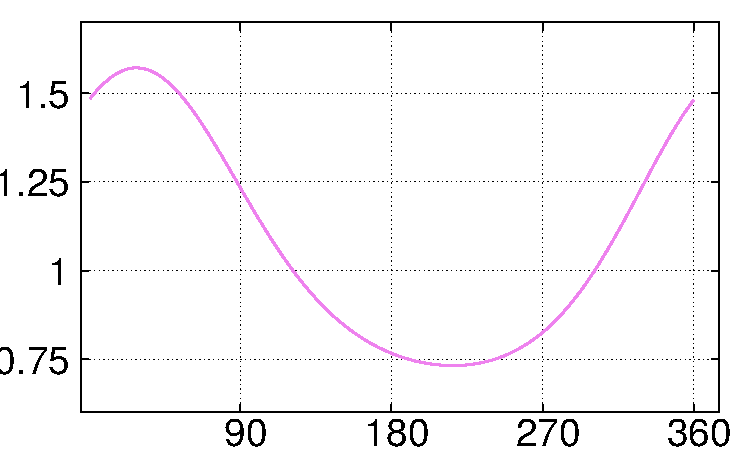
\includegraphics[width=0.38\textwidth]{part2/manovellismi/FIG/manovellismi/vel_b_infinito.pdf}
\end{center}
\begin{picture}(0,0)(0,0)
\scriptsize{
\put(55,70){${\omega_{\scalebox{.5}{DC}}}/{\omega_{\scalebox{.5}{AK}}}$}
        \put(141,27){$\alpha$}
}
\end{picture}
\vskip -3.2mm
      \caption{\em Velocit\`a del membro $DC$.}
     \label{fig:vel_b_infinito}
\end{wrapfigure}
\noindent Non \`e difficile, adottando
opportune configurazioni, ottenere per tale meccanismo un glifo
 rotante (sempre che
la volont\`a del progettista lo foggi come un glifo). L'analisi
qualitativa di tali meccanismi sar\`a oggetto di questo paragrafo.
\noindent Mandiamo
all'infinito la cerniera $B$ di un opportuno quadrilatero di partenza,
avente geometria tale da poter funzionare (si riveda la regola di {\em Grashof})
 a ``doppia-manovella''.
Abbiamo scelto la cerniera $B$ anzich\'e la $C$ semplicemente per
mostrare al lettore la completa equivalenza, in questa circostanza,
 delle
due cerniere. Nella nostra analisi, che svolgeremo come abbiamo fatto
altre volte tramite l'approccio numerico,
la manovella a velocit\`a costante \`e sempre la $AB$, che lascia
le sue tracce equispaziate; questo ci
consentir\`a di avere sulla manovella $DC$, l'elemento che di solito
\`e costituito da un glifo come in figura \ref{fig:glifo_rotante},
la velocit\`a variabile.
 
\begin{figure}[htb]
\begin{center}
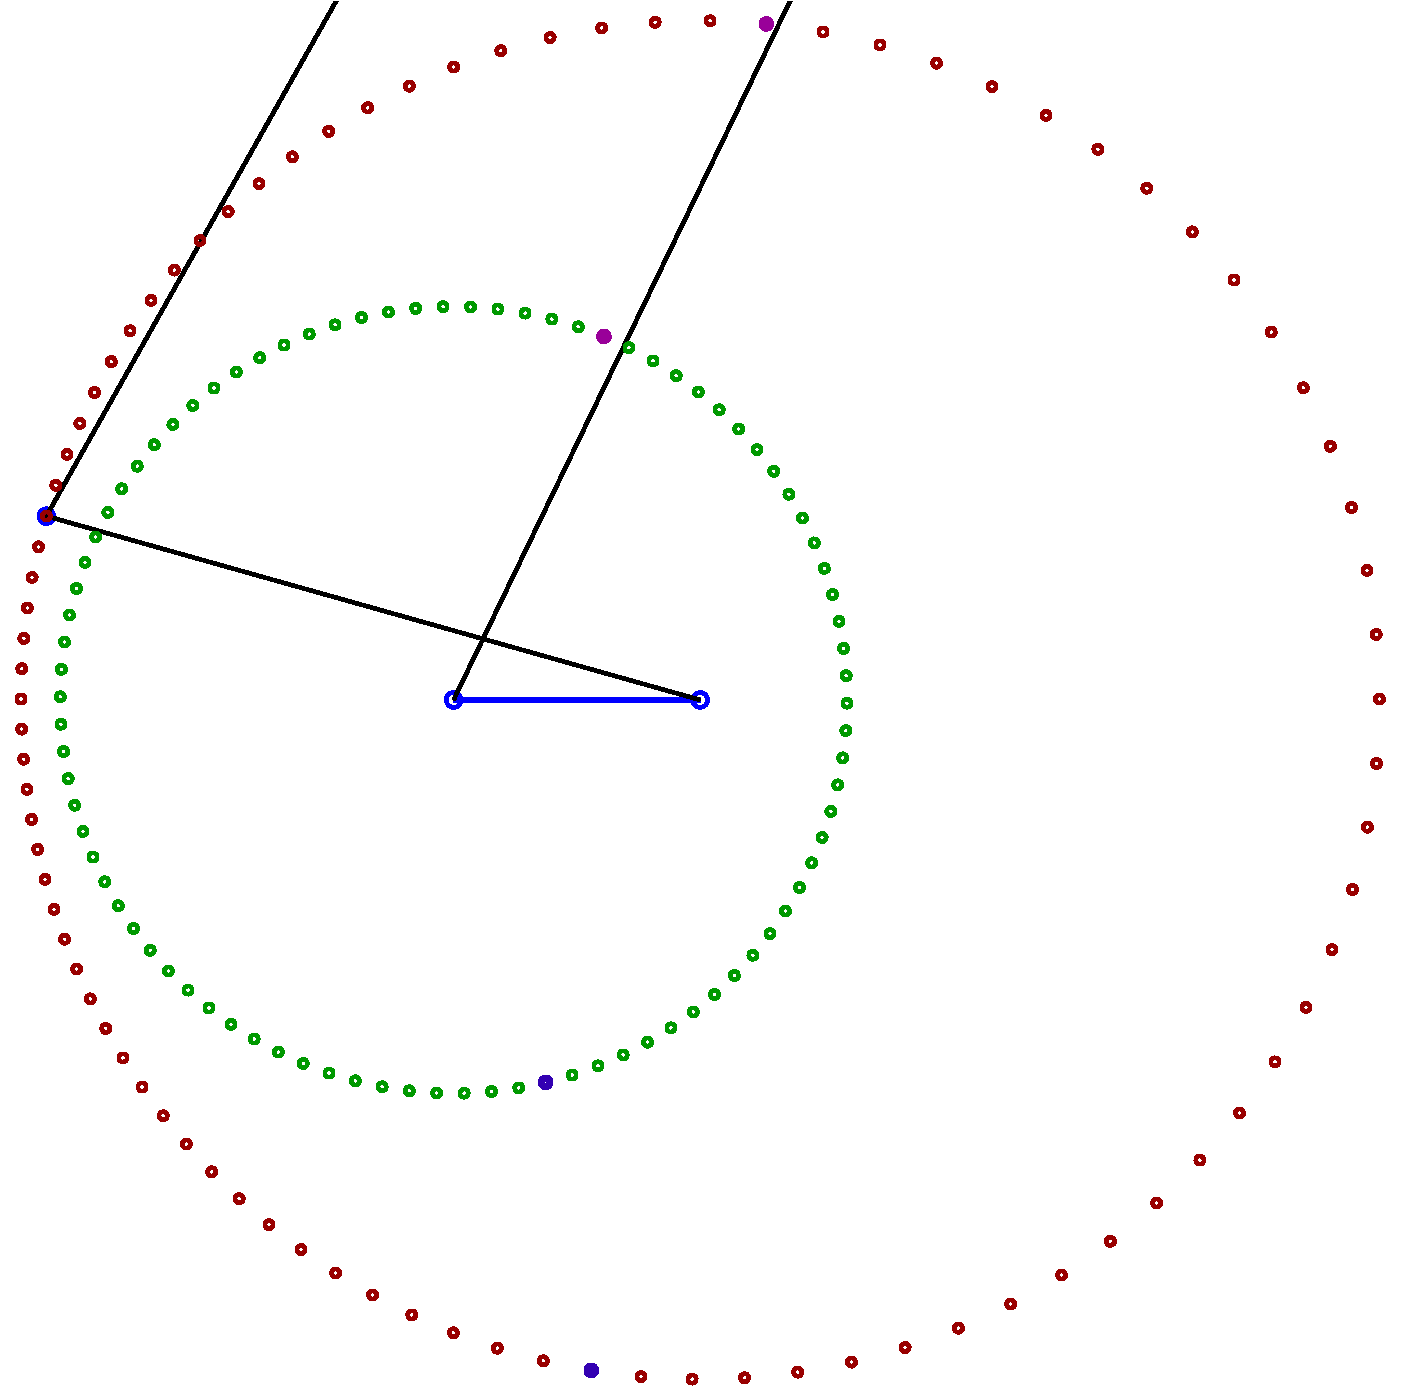
\includegraphics[width=.8\textwidth]{part2/manovellismi/FIG/manovellismi/b_infinito.pdf}
\end{center}
\begin{picture}(0,0)(-35,20)
\scriptsize{
\put(92,330){$B$}
\put(100,330){\rotatebox{67}{$\longrightarrow$}}
\put(104,328){$\infty$}
\put(-2,225){$C$}
\put(21,212){$K$}
\put(88,177){$A$}
\put(142,177){$D$}
\put(154,332){$\beta_2=86^{\circ}$}
\put(135,259){$\alpha_2=68^{\circ}$}
\put(115,100){$\alpha_1=292^{\circ}$}
\put(121,38){$\beta_1=274^{\circ}$}
}
\end{picture}
\vskip -3mm
      \caption{\em Manovellismo non ordinario che permette la rotazione completa
di due membri.}
 \label{fig:b_infinito}
\end{figure}

\noindent In particolare, la figura \ref{fig:vel_b_infinito} riporta l'andamento
del rapporto tra la velocit\`a angolare del glifo, $\omega_{DC}$, e quella
della manovella (presente nella figura \ref{fig:glifo_rotante}), $\omega_{AK}$.
Se volessimo valorizzare il massimo squilibrio che si pu\`o ottenere
tra la rotazione della manovella e quella del glifo,
come abbiamo esposto nel paragrafo {\ref{q_squilibrio}},
dovremmo anche qui trovare una posizione ben
precisa ``di montaggio'' di questo meccanismo.
Quest'ultimo quindi, se opportunamente sfruttato, potr\`a presentare, a fronte di due
semi-rotazioni contigue di $180^{\circ}$ del glifo, due angoli di manovella
sensibilmente diversi tra loro.
\begin{figure}[b]
\begin{center}
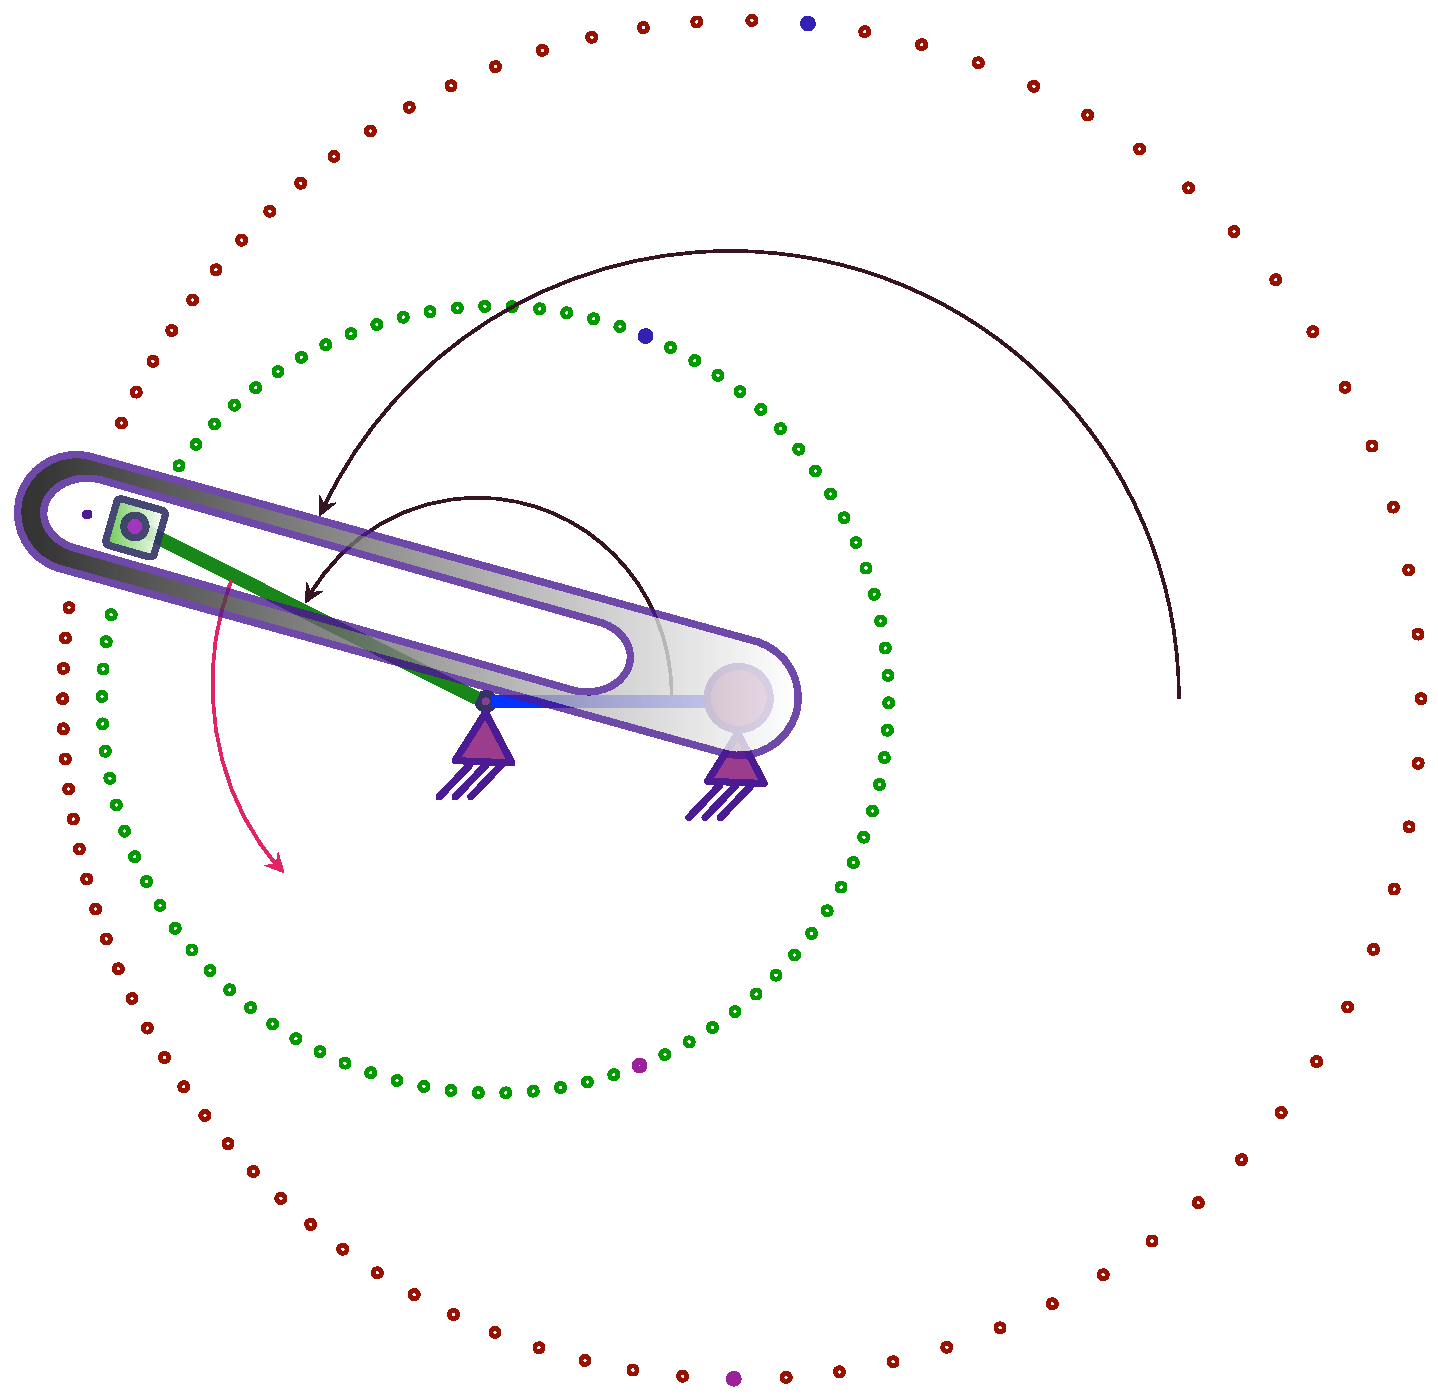
\includegraphics[width=.8\textwidth]{part2/manovellismi/FIG/glifo_rotante.pdf}
\end{center}
\begin{picture}(0,0)(-35,20)
\scriptsize{
\put(12,222){$C$}
\put(34,219){$K$}
\put(88,179){$A$}
\put(163,183){$D$}
\put(180,274){$\beta$}
\put(100,230){$\alpha$}
\put(52,142){$\omega={\rm cost}$}
}
\end{picture}
\vskip -5mm
      \caption{\em Manovellismo non ordinario 
 con glifo rotante.}
 \label{fig:glifo_rotante}
\end{figure}
 Riferendoci all'esempio di figura
\ref{fig:b_infinito}, figura sulla quale si 
basa quella successiva, \ref{fig:glifo_rotante}, 
troviamo indicate le coppie di angoli
$\alpha_1$, $\beta_1$, $\alpha_2$, $\beta_2$ che realizzano in questo caso
il {\em massimo squilibrio} pari a
\begin{equation}
s={{292^{\circ}-68^{\circ}}\over{360^{\circ} -292^{\circ} +68^{\circ}}} = 1.6\,.
\label{eq:esempio_squilibrio_glifo}
\end{equation} 
\noindent A una rotazione completa della manovella $AK$, a velocit\`a costante,
corrisponderanno quindi due semi-rotazioni del glifo che si completeranno
in tempi diversi tra loro con $t_a/t_r=1.6$. Si potrebbe quindi impiegare questo
glifo come manovella di
un manovellismo ordinario centrato, per il quale le corse di andata e ritorno
si svolgerebbero in tempi il cui rapporto reciproco \`e stato or ora indicato. 
Questa soluzione \`e stata talvolta adottata (glifo di {\em Whitworth}) in sostituzione
del glifo di {\em Fairbairn}, \cite{sesini1}, pag. 109.

\section{Quadrilateri Doppiamente Degeneri e Altre Considerazioni}

Tratteremo brevemente soltanto il caso in cui, spostando le due cerniere mobili,
$B$ e $C$, in due punti impropri distinti del piano, si d\`a luogo
a un interessante meccanismo di discreta importanza nelle applicazioni pratiche:
il {\em giunto di {\em Oldham}}\index{giunto di Oldham}.
La figura \ref{fig:oldham} mostra un quadrilatero a doppia-manovella
dove il telaio $AD$ misura circa la ventesima parte delle altre aste.
Siamo costretti, si fa per dire, a svelare ora l'arcano che sta alla base
delle figure dei manovellismi riportati in questo capitolo.
\begin{figure}[htb]
\begin{center}
\vspace{-0cm}\hspace{-.10cm}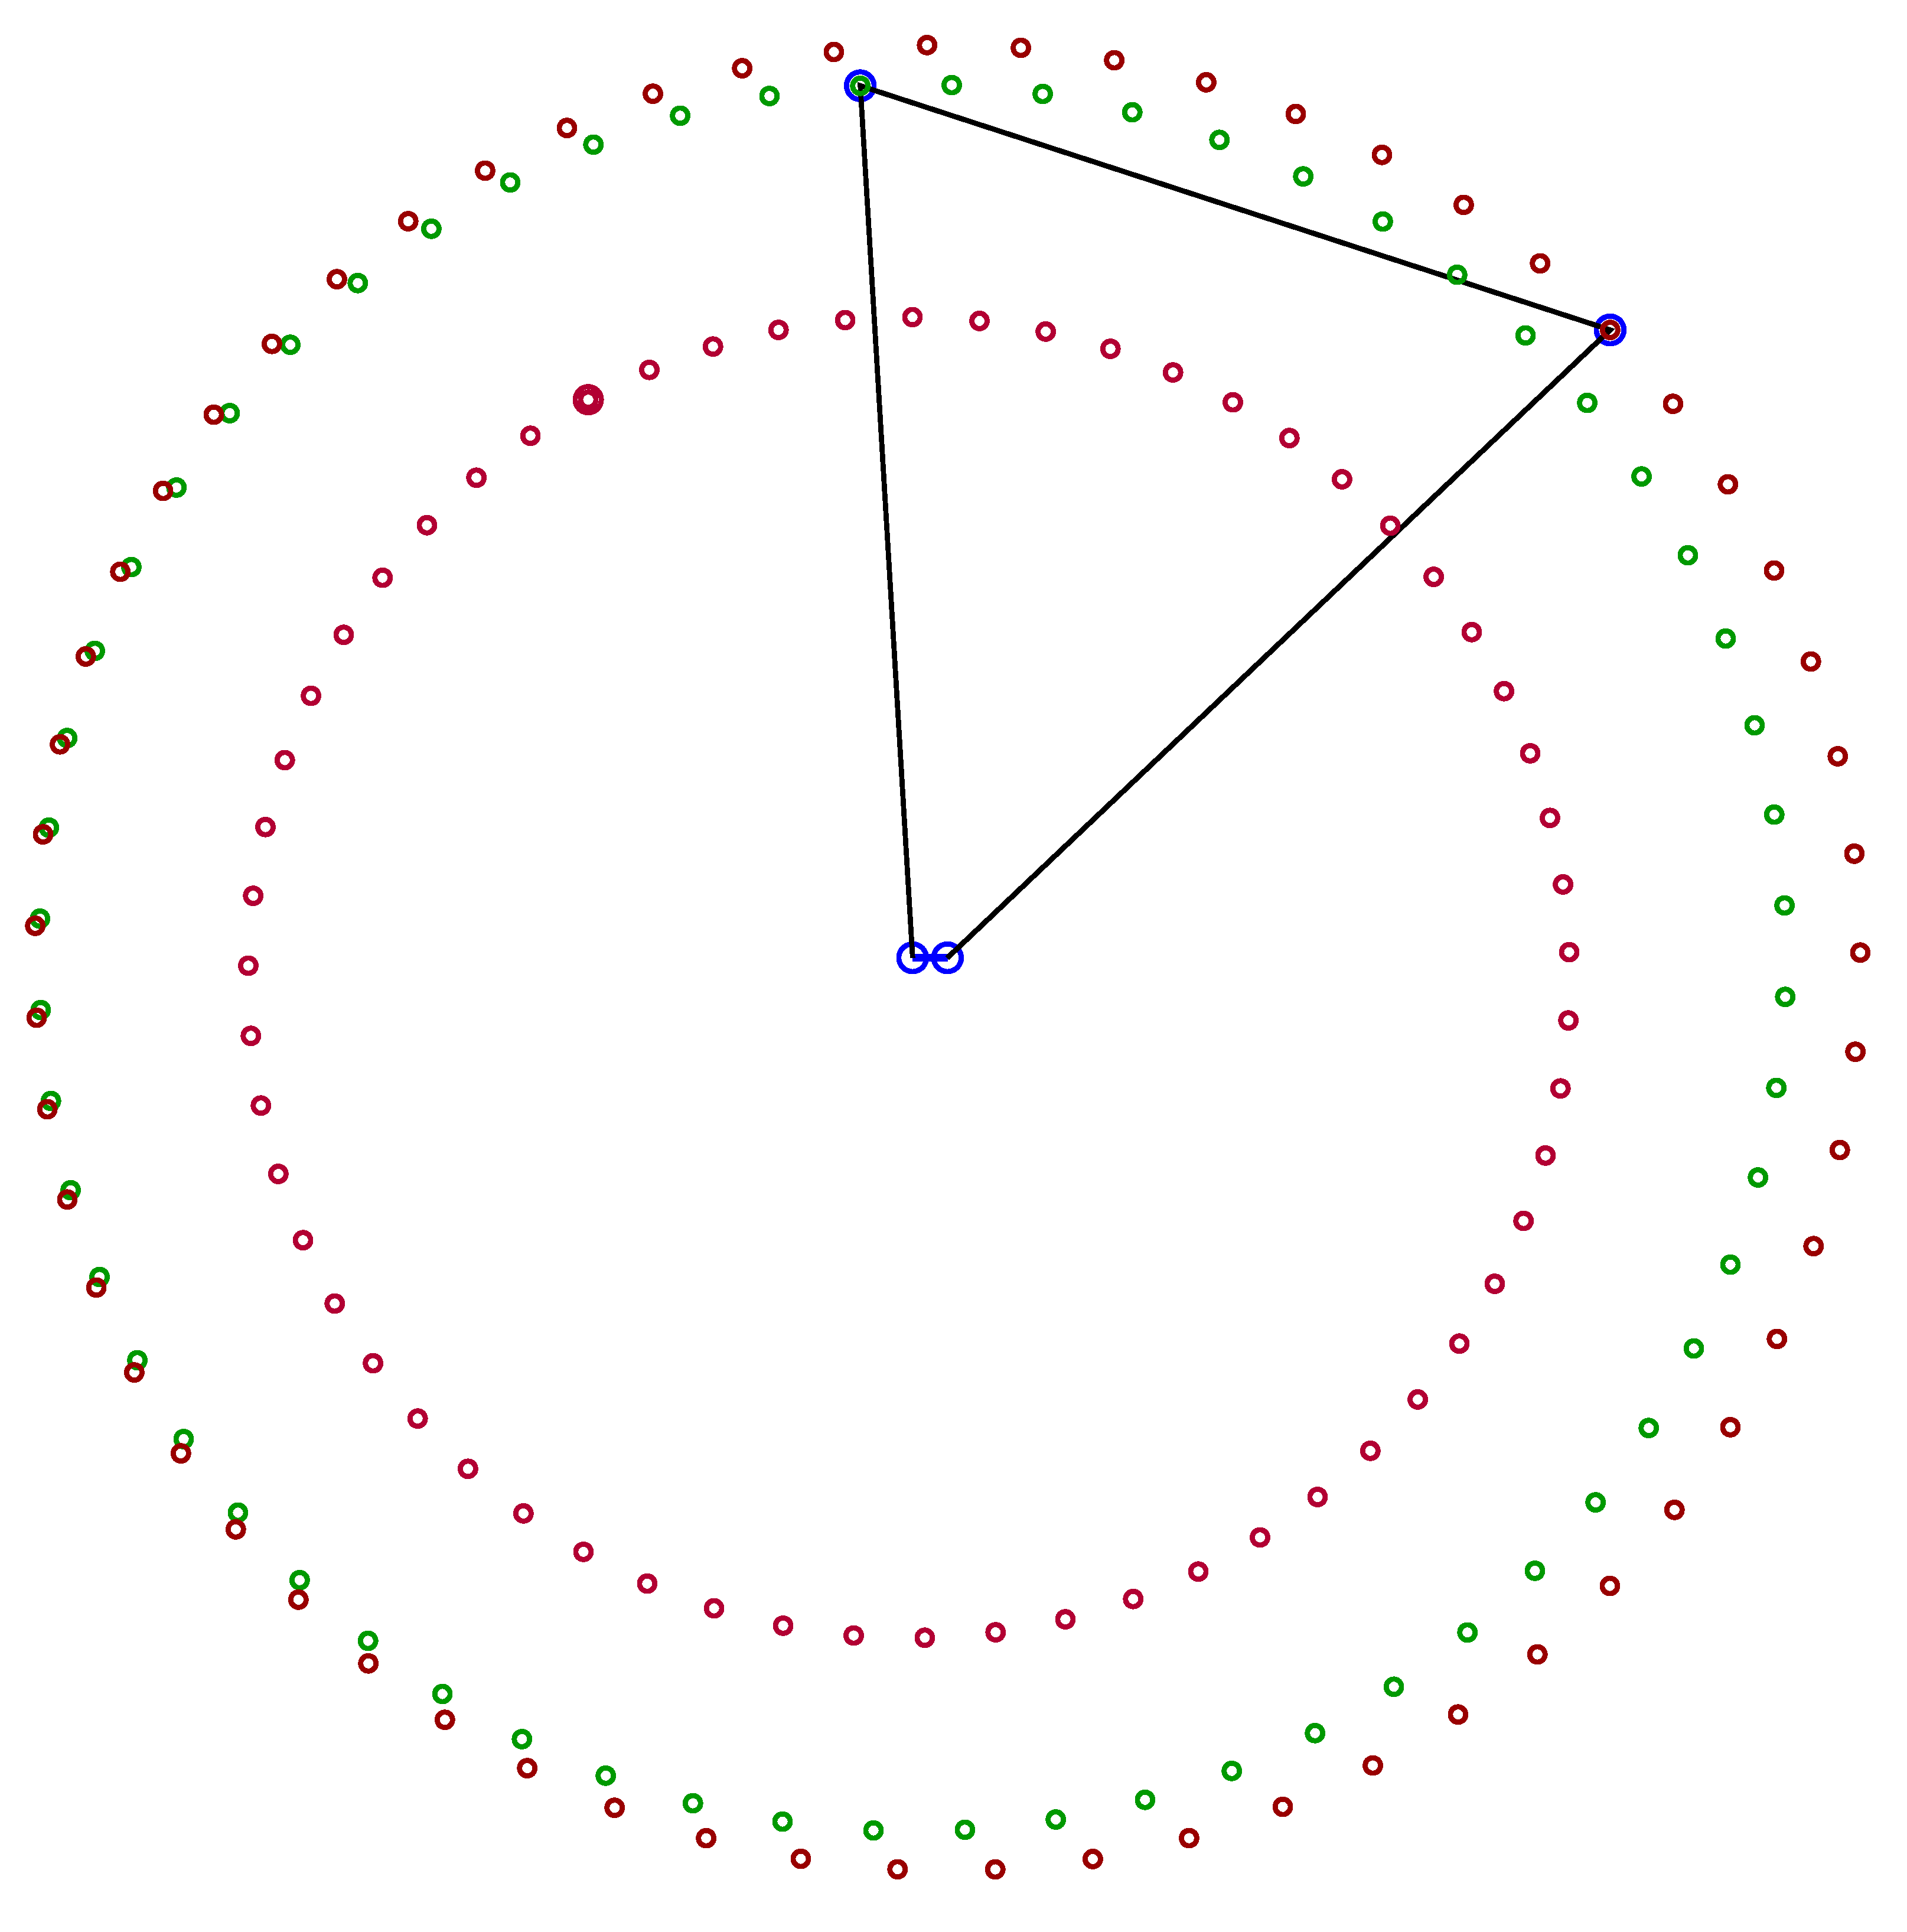
\includegraphics[width=.8\textwidth]{part2/manovellismi/FIG/manovellismi/oldham.pdf}
\hbox{\vspace{-12cm}\hspace{-4cm}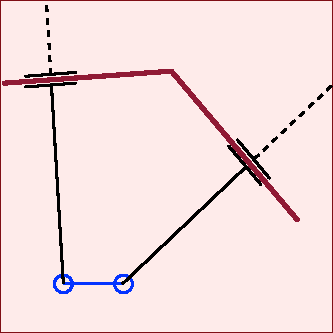
\includegraphics[width=0.3\textwidth]{part2/manovellismi/FIG/oldham_particolare.pdf}}
\end{center}
\begin{picture}(0,0)(-55,15)
\scriptsize{
\put(102,333){$B$}
\put(110,330){\rotatebox{90}{$\longrightarrow$}}
\put(114,333){$\infty$}
\put(232,293){$C$}
\put(234,287){\rotatebox{43.4}{$\longrightarrow$}}
\put(232,283){$\infty$}
\put(111,178){$A$}
\put(125,178){$D$}
\put(175,45){$A$}
\put(198,45){$D$}
\put(205,128){$T$}
\put(72,264){$P$}
}
\end{picture}
\vskip -5mm
      \caption{\em Quadrilatero doppiamente degenere e relativo meccanismo equivalente.
}
 \label{fig:oldham}
\end{figure}
Di fatto,
le analisi numeriche che danno origine alle figure \ref{fig:quad_D_infinito_man},
\ref{fig:c_infinito}, \ref{fig:c_infinito_quick} e \ref{fig:b_infinito} sono
state eseguite mediante lo  stesso (semplice e imperfetto) codice che genera
anche le analisi dei quadrilateri del precedente capitolo dedicato
allo studio dei quadrilateri articolati. In ambito numerico,
esiste infatti la possibilit\`a di analizzare, a volte con un certo agio,
anche quelle situazioni limite lasciate
giustamente dalla matematica nella sfera delle idee astratte, come sono in
generale le grandezze che tendono all'infinito.
Inoltre, le scienze ingegneristiche, pur abbracciando senza perplessit\`a il
concetto di distanza infinita, possono in altri casi permettersi il 
lusso  di accontentarsi di qualcosa di meno e magari pi\`u a portata di mano.
\`E il nostro caso, quando pretendiamo di trattare numericamente
le lunghezze, teoricamente infinite, delle aste $AD$ e $CD$ del quadrilatero
di figura \ref{fig:quad_D_infinito_man} sostituendo tali membri con
aste di lunghezza finita, bench\'e 
cinquanta o sessanta volte maggiore rispetto alle altre due.
Del resto, a nessun ingegnere di buon senso verrebbe in mente di obiettare
che la traiettoria del cursore, in figura \ref{fig:quad_D_infinito_man},
indicata con $\sigma$,
sia un arco di circonferenza anzich\'e un segmento di retta.
Torniamo alla figura \ref{fig:oldham} e  notiamo che la manovella $CD$
\`e omocinetica alla $AB$ (nell'approssimazione numerica adottata per le
lunghezze infinite delle tre aste $AB$, $BC$, e $CD$), cio\`e le due manovelle
hanno la stessa velocit\`a angolare.
La curva percorsa dal generico punto di biella $P$ approssimer\`a
tanto meglio una circonferenza quanto pi\`u distante si trover\`a dal telaio
(come nella figura) e anch'essa risulta percorsa con velocit\`a di modulo
costante. Risulta poi evidente che le curve di biella dei punti giacenti
(punti non rappresentati in figura per evitare confusione nel disegno)
 sulle manovelle, taglieranno queste ultime
seguendo direzioni ad esse ortogonali\footnote{\`E facile convincersi
che passando a lunghezze delle tre aste $AB$, $BC$ e $CD$ cento volte
superiori a quelle rappresentate  nella figura, i punti $A$ e $D$ verrebbero
a coincidere nel disegno in un punto $V$. Il meccanismo diventerebbe cos\`i
un triangolo $\triangle VBC$ che ruota attorno al suo vertice trascinando
in questa rotazione, oltre alle due manovelle, tutto il piano di biella.}.
\begin{figure}[hbt]
\centering
\begin{minipage}[b]{0.48\textwidth}
\centering
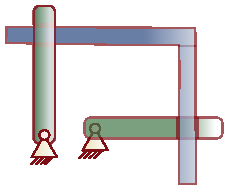
\includegraphics[width=0.95\textwidth]{part2/manovellismi/FIG/oldham_schema.pdf}
\begin{picture}(0,0)(190,0)
\scriptsize{
\put(36,40){$A$}
\put(48,75){$\scriptstyle{M_1}$}
\put(105,45){$\scriptstyle{M_2}$}
\put(110,110){$T$}
\put(85,57){$D$}
\put(116.5,57.5){$\omega$}
\put(35,51){$\omega$}
\put(33,54){\rotatebox{30}{$\curvearrowleft$}}
\put(110,62){\rotatebox{-60}{$\curvearrowleft$}}
}
\end{picture}
      \caption{\em Rappresentazione funzionale del giunto di Oldham.}
 \label{fig:oldham_schema}
\end{minipage}\hfill
\begin{minipage}[b]{0.48\textwidth}
\centering
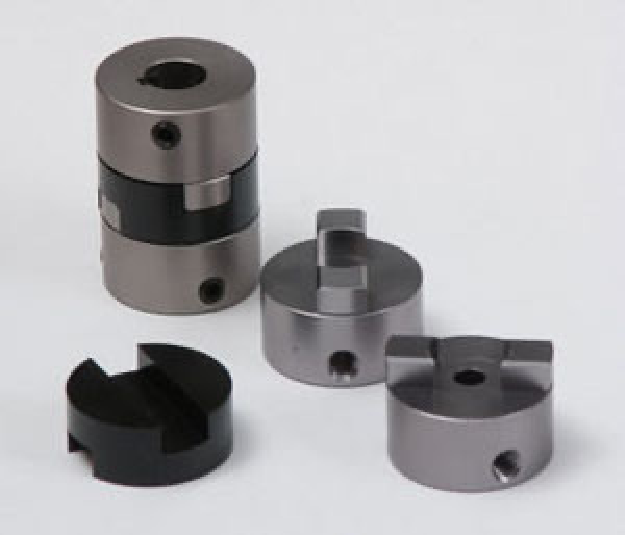
\includegraphics[width=0.95\textwidth]{part2/manovellismi/FIG/oldham_commerciale.pdf}
\begin{picture}(0,0)(100,0)
\scriptsize{
\put(30,80){$\scriptstyle{M_1}$}
\put(65,54){$\scriptstyle{M_2}$}
\put(-6,28){$T$}
}
\end{picture}
	\caption{\em Giunto di Oldham commerciale che permette disassamenti tra gli alberi fino a $5\, {\rm mm}$.}
     \label{fig:oldham_commerciale}
\end{minipage}
\end{figure}
\noindent Nel riquadro in basso a destra
della figura \ref{fig:oldham} \`e riportato un meccanismo equivalente
al quadrilatero doppiamente degenere che stiamo analizzando e 
la trave $T$ 
di tale figura riproduce quindi il comportamento della
biella $BC$.
\noindent Si intravede cos\`i la possibilit\`a di trasmettere
omocineticamente il moto
tra due alberi paralleli e tra loro disassati. In figura \ref{fig:oldham_schema}
\`e riportato un {\em giunto di Oldham} che presenta la trave $T$ come
una squadra. Questa soluzione \`e suggerita dal fatto che appare come privo di
senso privilegiare particolari direzioni radiali in un dispositivo il cui
funzionamento spazia su giri completi. D'altra
parte anche la posizione delle due ``chiavi'' pu\`o essere ottimizzata in modo
da diminuire l'ingombro complessivo. La figura \ref{fig:oldham_commerciale}
mostra un piccolo giunto di {\em Oldham} commerciale, dove i glifi sono stati
ricavati sulla trave $T$ e non sulle due manovelle; la figura mostra 
i tre componenti disgiunti, le due manovelle e la trave di collegamento,
nonch\'e il giunto
assemblato che dovrebbe convincere il lettore
della sua semplicit\`a e compattezza.

\noindent Come promesso nel titolo del presente paragrafo, esponiamo
qualche ulteriore considerazione circa i manovellismi e la loro classificazione
in ordinari e non ordinari. Nel percorso che abbiamo seguito in questo lavoro
viene evidenziata la differente genesi delle due tipologie di manovellismo:
quando a divenire un punto improprio \`e una delle due cerniere fisse
si ottiene un manovellismo ordinario, viceversa
si ottiene un manovellismo non ordinario quando a diventare impropria \`e
una delle altre due cerniere.  Mentre nella sfera delle applicazioni
pratiche la scelta del ``membro telaio'' \`e tutt'altro che indifferente (a
ben pochi \`e venuto in mente di costruire un motore dove a ruotare fosse
il blocco dei cilindri),
nell'ambito della cinematica teorica possiamo individuare soltanto
i moti relativi tra
le varie parti di un quadrilatero o di un manovellismo. In altre parole,
considerando di nuovo il manovellismo ordinario di figura \ref{fig:man_ord}
e tirando in ballo la nostra ormai affezionata formica esploratrice
(ve la ricordate? Quella della giostra dei cavalli...), potremmo
affermare che tale insetto vedrebbe un manovellismo ordinario quando
sta fermo sul glifo (il cilindro), un manovellismo non ordinario 
come quello di figura \ref{fig:c_infinito_equivalenti}- $3)$ quando
sta fermo sulla manovella $AB$ e un meccanismo equivalente a quello di
figura  \ref{fig:c_infinito_equivalenti}- $1)$ quando la formica sta ferma 
sulla biella $BC$. 
Questo punto di vista circa i diversi manovellismi,
che riteniamo chiarificatore e
didattico, viene esposto in molti libri che trattano questo argomento come,
ad esempio, \cite{sesini1}, pag. 107.
%\newpage
%\thispagestyle{empty}
%\null
\endinput 
